\documentclass[16pt]{beamer}
\usepackage{algorithm}
\usepackage{algorithmic}
\usepackage[numbers]{natbib}
\usepackage{pgf,pgfarrows,pgfnodes}
% \usepackage{beamerthemesplit} // Activate for custom appearance

\title{Stochastic memoization, Bayesian nonparametrics, and the goal of developing general-purpose predictive models}
\author{Frank Wood \\\qquad \\ joint work with Nicholas Bartlett, David Pfau, Jan Gasthaus, C\'{e}dric Archambeau, Lancelot James, Yee Whye Teh, and more...}
\date{\today}



\usetheme{Darmstadt}
%\usetheme{Copenhagen}
%\usefonttheme[onlylarge]{structurebold}
%\setbeamerfont*{frametitle}{size=\normalsize,series=\bfseries}
%\setbeamertemplate{navigation symbols}{}

\usepackage{amsfonts}
\usepackage{amsmath}
%\newcommand{\argmax}{\operatornamewithlimits{argmax}}
\def\newblock{\hskip .11em plus .33em minus .07em}
% Setup TikZ

% !TEX root = talk.tex

\newcommand{\comment}[1]{}
%\newcommand{\comment}[1]{{\marginpar{\tiny {#1} }}}
\def\todo#1{TODO(#1)}

\def\bigO{{\mathcal O}}
\def\balpha{\mbox{\boldmath $\alpha$}}
\def\bbeta{\mbox{\boldmath $\beta$}}
\def\beeta{\mbox{\boldmath $\eta$}}
\def\blambda{\mbox{\boldmath $\lambda$}}
\def\bmu{\mbox{\boldmath $\mu$}}
\def\bphi{\mbox{\boldmath $\phi$}}
\def\bpsi{\mbox{\boldmath $\psi$}}
\def\bsigma{\mbox{\boldmath $\sigma$}}
\def\btau{\mbox{\boldmath $\tau$}}
\def\btheta{\mbox{\boldmath $\theta$}}
\def\dbphi{\dot{\mbox{\boldmath $\phi$}}}
\def\dbtau{\dot{\mbox{\boldmath $\tau$}}}
\def\dbtheta{\dot{\mbox{\boldmath $\theta$}}}

%\newcommand{\nofootnotemark}{\let\@makefnmark\relax}
\newcommand{\bX}{\mathbf{X}}
\newcommand{\bY}{\mathbf{Y}}
\newcommand{\bW}{\mathbf{W}}
\newcommand{\bZ}{\mathbf{Z}}
\newcommand{\bH}{\mathbf{H}}
\newcommand{\bQ}{\mathbf{Q}}
\newcommand{\bA}{\mathbf{A}}
\newcommand{\bI}{\mathbf{I}}
\newcommand{\by}{\mathbf{y}}
\newcommand{\bz}{\mathbf{z}}
\newcommand{\bx}{\mathbf{x}}

\newcommand{\ith}{i^\mathrm{th}}
\def\A{{\bf A}}
\def\B{{\bf B}}
\def\C{{\bf C}}
\def\D{{\bf D}}
\def\F{{\bf F}}
\def\L{{\bf L}}
\def\M{{\bf M}}
\def\W{{\bf W}}
\def\I{{\bf I}}
\def\J{{\bf J}}
\def\R{{\bf R}}
\def\U{{\bf U}}
\def\V{{\bf V}}
\def\b{{\bf b}}
\def\c{{\bf c}}
\def\d{{\bf d}}
\def\r{{\bf r}}
\def\s{{\bf s}}
\def\t{{\bf t}}
\def\u{{\bf u}}
\def\v{{\bf v}}
\def\f{{\bf f}}
\def\x{{\bf x}}
\def\y{{\bf y}}
\def\w{{\bf w}}
\def\vo{{\bf o}}
\def\p{{\bf p}}
\def\O{{\bf 0}}
%\def\a{{\bf a}}


\def\vbpsi{\vec{\mbox{\boldmath $\psi$}}} 
\def\vpsi{\vec{\psi}} 
\def\vbphi{\vec{\mbox{\boldmath $\phi$}}} 
\def\vphi{\vec{\phi}} 
\def\vbtau{\vec{\mbox{\boldmath $\tau$}}} 
\def\vbtheta{\vec{\mbox{\boldmath $\theta$}}} 
\def\vD{\vec{D}}
\def\vf{\vec{\bf f}}
\def\vF{\vec{\bf F}}
\def\vI{\vec{\bf I}}
\def\vR{\vec{\bf R}}
\def\vv{\vec{v}}
\def\vV{\vec{\bf V}}

\def\pon{p_{\mathrm{on}}}
\def\poff{p_{\mathrm{off}}}

\def\tr{^{\text{T}}}

%%% Vector notation for sections 3 and 4
%%% Vector notation for sections 3 and 4
\def\mvec{\vec{m}}
\def\fvec{\vec{f}}
\def\appfvec{\vec{f}_k}
\def\avec{\vec{a}}
\def\bvec{\vec{b}}
\def\evec{\vec{e}}
\def\uvec{\vec{u}}
\def\xvec{\vec{x}}
\def\wvec{\vec{w}}
\def\gradvec{\vec{\nabla}}

\def\aM{\mbox{\bf a}_M}
\def\aS{\mbox{\bf a}_S}
\def\aO{\mbox{\bf a}_O}
\def\aL{\mbox{\bf a}_L}
\def\aP{\mbox{\bf a}_P}
\def\ai{\mbox{\bf a}_i}
\def\aj{\mbox{\bf a}_j}
\def\an{\mbox{\bf a}_n}
\def\a1{\mbox{\bf a}_1}
\def\a2{\mbox{\bf a}_2}
\def\a3{\mbox{\bf a}_3}
\def\a4{\mbox{\bf a}_4}

%\def\x{\mbox{\bf x\/}}
%\def\X{\mbox{\bf X}}
%\def\A{\mbox{\bf A}}
%\def\P{\mbox{\bf P}}
%\def\C{\mbox{\bf C}}
%\def\c{\mbox{\bf c}}
%\def\b{\mbox{\bf b}}
%\def\o{\mbox{\bf o}}
%\def\h{\mbox{\bf h}}
%\def\f{\mbox{\bf f}}
%\def\x{\mbox{\bf x}}
%\def\sx{\mbox{\scriptsize\bf x}}
%\def\z{\mbox{\bf z}}
%\def\l{\mbox{\bf l}}
%\def\m{\mbox{\bf m}}
%\def\bi{\mbox{\bf i}}
%\def\u{\mbox{\bf u}}
%\def\v{\mbox{\bf v}}
\def\a{\mbox{\bf a}}
%\def\p{\mbox{\bf p}}
%\def\r{\mbox{\bf r}}
%\def\d{\mbox{\bf d}}
%\def\Q{\mbox{\bf Q}}
%\def\s{\mbox{\bf s}}
%\def\st{\mbox{\scriptsize\bf t}}
%\def\ss{\mbox{\scriptsize\bf s}}
%\def\t{\mbox{\bf t}}
%\def\cR{{\cal R}}
%\def\calD{{\cal D}}
%\def\calS{{\cal S}}
%\def\g{\mbox{\bf g}}
%\def\e{\mbox{\bf e}}
%\def\flow{\{\mbox{\bf u}\}}
%\def\appearChange{iconic change}

\def\sigmae{\sigma}
\def\sigmam{\sigma}

\newcommand{\eg}{e.\thinspace{}g.,\@\xspace}
\newcommand{\egn}{e.\thinspace{}g.\@\xspace}
\newcommand{\cf}{cf.\@\xspace}
\newcommand{\ie}{i.\thinspace{}e.,\@\xspace}
\newcommand{\ien}{i.\thinspace{}e.\@\xspace}
\newcommand{\iid}{i.\thinspace{}i.\thinspace{}d.\@\xspace}


%\newcommand{\comment}[1]{}
\newcommand{\ponedec}{\mathcal{P}^\downarrow_1}
\newcommand{\pone}{\mathcal{P}_1}
\newcommand{\rank}[1]{\mathrm{RANK}\left[#1\right]}
\newcommand{\E}[1]{\mathrm{E}\left[#1\right]}
%\newcommand{\PY}{\mathcal{PY}}
%\newcommand{\DP}{\mathcal{DP}}
%\newcommand{\iid}{iid.}
\newcommand{\drawiid}{\stackrel{\text{iid}}{\sim}}
\newcommand{\vect}[1]{\mathbf{#1}}
\newcommand{\indicator}[1]{\text{I}\left[ #1 \right]}
\newcommand{\pdcoag}{PD(d_1,0)-\text{COAG}}
%\newcommand{\todo}{\textbf{*TODO*}}
\newcommand{\igram}{\text{$\infty$-gram}}
\newcommand{\Prob}{\text{P}}

\def\mm{sequence memoizer }
\def\MM{SM }

\def\pibf{{\boldsymbol{\pi}}}
\def\kapbf{\boldsymbol{\kappa}}
\def\taubf{\boldsymbol{\tau}}
\def\thebf{\boldsymbol{\theta}}
\def\rhobf{\boldsymbol{\rho}}
\def\phibf{\boldsymbol{\phi}}
\def\pbf{\mathbf{p}}
\def\qbf{\mathbf{q}}
\def\sbf{\mathbf{s}}
\def\tbf{\mathbf{t}}
\def\ybf{\mathbf{y}}
\def\ubf{\mathbf{u}}
\def\Ave{\mathbb{E}}

\def\wbf{\mathbf{w}}
\def\xbf{\mathbf{x}}
\def\rbf{\mathbf{r}}
\def\tbf{\mathbf{t}}
\def\kbf{\mathbf{k}}
\def\Xbf{\mathbf{X}}
\def\0bf{\mathbf{0}}
\def\Ibf{\mathbf{I}}
\def\phibf{\mathbf{\phi}}
\def\Phibf{\mathbf{\Phi}}
\def\disteq{{\stackrel{D}{=}}}
\def\EE{{\mathbb{E}}}
\def\GG{\mathcal{G}}
\def\G{G}
\def\U{U}

\def\phiv{\varphi}
\def\phivbf{\boldsymbol{\varphi}}

\def\Ocal{\mathcal{O}}
\DeclareMathOperator*{\Var}{Var}

\DeclareMathOperator*{\Bet}{Beta}
\DeclareMathOperator{\coag}{COAG}
\DeclareMathOperator{\frag}{FRAG}
\DeclareMathOperator*{\rnk}{RANK}
\DeclareMathOperator*{\gem}{GEM}
\DeclareMathOperator*{\pd}{PD}
\DeclareMathOperator*{\py}{PY}
\DeclareMathOperator*{\DP}{DP}
\DeclareMathOperator*{\PY}{PY}
\DeclareMathOperator*{\gd}{GDir}
\DeclareMathOperator*{\Dir}{Dir}
\DeclareMathOperator*{\CRP}{CRP}
\DeclareMathOperator*{\argmax}{argmax}



%%% Local Variables: 
%%% mode: latex
%%% TeX-master: "paper"
%%% End: 
% !TEX root = talk.tex
%
%\newcommand{\comment}[1]{}
%%\newcommand{\comment}[1]{{\marginpar{\tiny {#1} }}}
%
%\def\bigO{{\mathcal O}}
%\def\balpha{\mbox{\boldmath $\alpha$}}
%\def\bbeta{\mbox{\boldmath $\beta$}}
%\def\beeta{\mbox{\boldmath $\eta$}}
%\def\blambda{\mbox{\boldmath $\lambda$}}
%\def\bmu{\mbox{\boldmath $\mu$}}
%\def\bphi{\mbox{\boldmath $\phi$}}
%\def\bpsi{\mbox{\boldmath $\psi$}}
%\def\bsigma{\mbox{\boldmath $\sigma$}}
%\def\btau{\mbox{\boldmath $\tau$}}
%\def\btheta{\mbox{\boldmath $\theta$}}
%\def\dbphi{\dot{\mbox{\boldmath $\phi$}}}
%\def\dbtau{\dot{\mbox{\boldmath $\tau$}}}
%\def\dbtheta{\dot{\mbox{\boldmath $\theta$}}}
%
%%\newcommand{\nofootnotemark}{\let\@makefnmark\relax}
%\newcommand{\bX}{\mathbf{X}}
%\newcommand{\bY}{\mathbf{Y}}
%\newcommand{\bW}{\mathbf{W}}
%\newcommand{\bZ}{\mathbf{Z}}
%\newcommand{\bH}{\mathbf{H}}
%\newcommand{\bQ}{\mathbf{Q}}
%\newcommand{\bA}{\mathbf{A}}
%\newcommand{\bI}{\mathbf{I}}
%\newcommand{\by}{\mathbf{y}}
%\newcommand{\bz}{\mathbf{z}}
%\newcommand{\bx}{\mathbf{x}}
%
%\newcommand{\ith}{i^\mathrm{th}}
%\def\A{{\bf A}}
%\def\B{{\bf B}}
%\def\C{{\bf C}}
%\def\D{{\bf D}}
%\def\F{{\bf F}}
%\def\L{{\bf L}}
%\def\M{{\bf M}}
%\def\W{{\bf W}}
%\def\I{{\bf I}}
%\def\J{{\bf J}}
%\def\R{{\bf R}}
%\def\U{{\bf U}}
%\def\V{{\bf V}}
%\def\b{{\bf b}}
%\def\c{{\bf c}}
%\def\d{{\bf d}}
%\def\r{{\bf r}}
%\def\s{{\bf s}}
%\def\t{{\bf t}}
%\def\u{{\bf u}}
%\def\v{{\bf v}}
%\def\f{{\bf f}}
%\def\x{{\bf x}}
%\def\y{{\bf y}}
%\def\w{{\bf w}}
%\def\vo{{\bf o}}
%\def\p{{\bf p}}
%\def\O{{\bf 0}}
%%\def\a{{\bf a}}
%
%
%\def\vbpsi{\vec{\mbox{\boldmath $\psi$}}} 
%\def\vpsi{\vec{\psi}} 
%\def\vbphi{\vec{\mbox{\boldmath $\phi$}}} 
%\def\vphi{\vec{\phi}} 
%\def\vbtau{\vec{\mbox{\boldmath $\tau$}}} 
%\def\vbtheta{\vec{\mbox{\boldmath $\theta$}}} 
%\def\vD{\vec{D}}
%\def\vf{\vec{\bf f}}
%\def\vF{\vec{\bf F}}
%\def\vI{\vec{\bf I}}
%\def\vR{\vec{\bf R}}
%\def\vv{\vec{v}}
%\def\vV{\vec{\bf V}}
%
%\def\pon{p_{\mathrm{on}}}
%\def\poff{p_{\mathrm{off}}}
%
%\def\tr{^{\text{T}}}
%
%%%% Vector notation for sections 3 and 4
%%%% Vector notation for sections 3 and 4
%\def\mvec{\vec{m}}
%\def\fvec{\vec{f}}
%\def\appfvec{\vec{f}_k}
%\def\avec{\vec{a}}
%\def\bvec{\vec{b}}
%\def\evec{\vec{e}}
%\def\uvec{\vec{u}}
%\def\xvec{\vec{x}}
%\def\wvec{\vec{w}}
%\def\gradvec{\vec{\nabla}}
%
%\def\aM{\mbox{\bf a}_M}
%\def\aS{\mbox{\bf a}_S}
%\def\aO{\mbox{\bf a}_O}
%\def\aL{\mbox{\bf a}_L}
%\def\aP{\mbox{\bf a}_P}
%\def\ai{\mbox{\bf a}_i}
%\def\aj{\mbox{\bf a}_j}
%\def\an{\mbox{\bf a}_n}
%\def\a1{\mbox{\bf a}_1}
%\def\a2{\mbox{\bf a}_2}
%\def\a3{\mbox{\bf a}_3}
%\def\a4{\mbox{\bf a}_4}
%
%%\def\x{\mbox{\bf x\/}}
%%\def\X{\mbox{\bf X}}
%%\def\A{\mbox{\bf A}}
%%\def\P{\mbox{\bf P}}
%%\def\C{\mbox{\bf C}}
%%\def\c{\mbox{\bf c}}
%%\def\b{\mbox{\bf b}}
%%\def\o{\mbox{\bf o}}
%%\def\h{\mbox{\bf h}}
%%\def\f{\mbox{\bf f}}
%%\def\x{\mbox{\bf x}}
%%\def\sx{\mbox{\scriptsize\bf x}}
%%\def\z{\mbox{\bf z}}
%%\def\l{\mbox{\bf l}}
%%\def\m{\mbox{\bf m}}
%%\def\bi{\mbox{\bf i}}
%%\def\u{\mbox{\bf u}}
%%\def\v{\mbox{\bf v}}
%\def\a{\mbox{\bf a}}
%%\def\p{\mbox{\bf p}}
%%\def\r{\mbox{\bf r}}
%%\def\d{\mbox{\bf d}}
%%\def\Q{\mbox{\bf Q}}
%%\def\s{\mbox{\bf s}}
%%\def\st{\mbox{\scriptsize\bf t}}
%%\def\ss{\mbox{\scriptsize\bf s}}
%%\def\t{\mbox{\bf t}}
%%\def\cR{{\cal R}}
%%\def\calD{{\cal D}}
%%\def\calS{{\cal S}}
%%\def\g{\mbox{\bf g}}
%%\def\e{\mbox{\bf e}}
%%\def\flow{\{\mbox{\bf u}\}}
%%\def\appearChange{iconic change}
%
%\def\sigmae{\sigma}
%\def\sigmam{\sigma}
%
%\newcommand{\eg}{e.\thinspace{}g.,\@\xspace}
%\newcommand{\egn}{e.\thinspace{}g.\@\xspace}
%\newcommand{\cf}{cf.\@\xspace}
%\newcommand{\ie}{i.\thinspace{}e.,\@\xspace}
%\newcommand{\ien}{i.\thinspace{}e.\@\xspace}
%\newcommand{\iid}{i.\thinspace{}i.\thinspace{}d.\@\xspace}
%
%
%%\newcommand{\comment}[1]{}
%\newcommand{\ponedec}{\mathcal{P}^\downarrow_1}
%\newcommand{\pone}{\mathcal{P}_1}
%\newcommand{\rank}[1]{\mathrm{RANK}\left[#1\right]}
%%\newcommand{\E}[1]{\mathrm{E}\left[#1\right]}
%%\newcommand{\PY}{\mathcal{PY}}
%%\newcommand{\DP}{\mathcal{DP}}
%%\newcommand{\iid}{iid.}
%\newcommand{\drawiid}{\stackrel{\text{iid}}{\sim}}
%\newcommand{\vect}[1]{\mathbf{#1}}
%\newcommand{\indicator}[1]{\text{I}\left[ #1 \right]}
%\newcommand{\pdcoag}{PD(d_1,0)-\text{COAG}}
%%\newcommand{\todo}{\textbf{*TODO*}}
%\newcommand{\igram}{\text{$\infty$-gram}}
%\newcommand{\Prob}{\text{P}}
%
%\def\mm{sequence memoizer }
%\def\MM{SM }
%
%\def\pibf{{\boldsymbol{\pi}}}
%\def\kapbf{\boldsymbol{\kappa}}
%\def\taubf{\boldsymbol{\tau}}
%\def\thebf{\boldsymbol{\theta}}
%\def\rhobf{\boldsymbol{\rho}}
%\def\phibf{\boldsymbol{\phi}}
%\def\pbf{\mathbf{p}}
%\def\qbf{\mathbf{q}}
%\def\sbf{\mathbf{s}}
%\def\tbf{\mathbf{t}}
%\def\ybf{\mathbf{y}}
%\def\ubf{\mathbf{u}}
%\def\Ave{\mathbb{E}}
%
%\def\wbf{\mathbf{w}}
%\def\xbf{\mathbf{x}}
%\def\rbf{\mathbf{r}}
%\def\tbf{\mathbf{t}}
%\def\kbf{\mathbf{k}}
%\def\Xbf{\mathbf{X}}
%\def\0bf{\mathbf{0}}
%\def\Ibf{\mathbf{I}}
%\def\phibf{\mathbf{\phi}}
%\def\Phibf{\mathbf{\Phi}}
%\def\disteq{{\stackrel{D}{=}}}
%\def\GG{\mathcal{G}}
%\def\G{G}
%\def\U{U}
%
%\def\phiv{\varphi}
%\def\phivbf{\boldsymbol{\varphi}}
%
%\def\Ocal{\mathcal{O}}
%\DeclareMathOperator*{\Var}{Var}
%
%\DeclareMathOperator*{\Bet}{Beta}
%\DeclareMathOperator{\coag}{COAG}
%\DeclareMathOperator{\frag}{FRAG}
%\DeclareMathOperator*{\rnk}{RANK}
%\DeclareMathOperator*{\gem}{GEM}
%\DeclareMathOperator*{\pd}{PD}
%\DeclareMathOperator*{\py}{PY}
%\DeclareMathOperator*{\DP}{DP}
%\DeclareMathOperator*{\PY}{PY}
%\DeclareMathOperator*{\gd}{GDir}
%\DeclareMathOperator*{\Dir}{Dir}
%\DeclareMathOperator*{\CRP}{CRP}
%\DeclareMathOperator*{\argmax}{argmax}
%
\def\GG{\mathcal{G}}
\def\data{\mathbf{x}}
%\def\EE{\mathbb{E}}
\def\disc{d}
%\newcommand{\delete}[1]{} %\textcolor{red}{#1}
%\newcommand{\rewrite}[1]{#1}%{\textcolor{blue}{#1}} %
%\newcommand{\lambdabf}{\boldsymbol{\lambda}}
%\newcommand{\vbf}{\mathbf{v}}
%\newcommand{\Psmooth}{\Prob_\text{smooth}}
%%\newcommand{\parent}{\pi}
%\newcommand{\suffix}{\sigma}
%\newcommand{\UHPYP}{SM}
%\newcommand{\PLUMP}{PLUMP}
%\newcommand{\Oh}{\mathcal{O}}
%\newcommand{\tree}{\mathcal{T}}
\newcommand{\cct}{\hat{\mathcal{T}}}
\newcommand{\cctx}{\cct(\data)}
\newcommand{\Gu}{G_{\ubf}}
%\newcommand{\GuSet}{\{G_{\ubf}\}_{\ubf \in \Sigma^*}}
%\newcommand{\E}{\mathrm{E}}
%\newcommand{\UpdatePath}{\text{\textsc{UpdatePath}}}
%\newcommand{\Path}{\ensuremath{(\ubf_0,\ldots,\ubf_P)}}
%\newcommand{\PathProbability}{\text{\textsc{PathProbability}}}
%\newcommand{\TT}{\mathcal{T}}
%\newcommand{\ral}[1]{\stackrel{\mathtt{#1}}{\rightarrow}}
\def\parent{{\sigma(\mathbf{u})}}
%
%%\def\newblock{\hskip .11em plus .33em minus .07em}
%
%
%% \newcommand{\cusk}{c_{\ubf s k}}
%% \newcommand{\cus}{c_{\ubf s \cdot}}
%% \newcommand{\cu}{c_{\ubf \cdot \cdot}}
%% \newcommand{\tus}{t_{\ubf s}}
%% \newcommand{\tu}{t_{\ubf \cdot}}
%\newcommand{\cusk}{c_{\ubf s k}}
%\newcommand{\cus}{c_{\ubf s}}
%\newcommand{\cu}{c_{\ubf \cdot}}
%\newcommand{\tus}{t_{\ubf s}}
%\newcommand{\tu}{t_{\ubf \cdot}}
%\newcommand{\cset}{\{\cusk\}_{s\in \Sigma,k \in \{1,\ldots,t_{\ubf s}\}}}
%\newcommand{\tset}{\{\tus\}_{s\in \Sigma}}
%\newcommand{\bydef}{\equiv}
%\newcommand{\state}{\mathcal{S}_{\xbf}}
%\newcommand{\statei}{\mathcal{S}_{\xbf_{1:i}}}
%%\newcommand{\emptystring}{\varepsilon}
%\newcommand{\gcount}{\hat{c}}
%\newcommand{\escape}{\mathtt{esc}}
%\def\prob{G}
%
%
%\newcommand{\todo}[1]{\begin{center}\textbf{TODO: } #1 \end{center}}
%\newcommand{\figref}[1]{\figurename~\ref{#1}}
%\newcommand{\predictive}{\Prob(x_i|\xbf_{1:i-1})}
%\newcommand{\ywcomment}[1]{\textbf{#1}}
%\newcommand{\jgcomment}[1]{ { \textcolor{red}{#1} } }
%
%\newcommand{\secref}[1]{Section \ref{#1}}
%
\def\context{\mathbf{u}}

%%% Local Variables: 
%%% mode: latex
%%% TeX-master: "paper"
%%% End: 



\title[Sequence Memoizer] 
{
	Stochastic memoization, Bayesian nonparametrics, and the goal of developing general-purpose predictive models
}

\author[http://www.stat.columbia.edu/$\sim$fwood]
{
  Frank~Wood \\ 
 \qquad \\
  {\small joint work with \\ \qquad \\ Nicholas Bartlett, David Pfau, Jan Gasthaus, C\'{e}dric Archambeau, Lancelot James, Yee Whye Teh, and more...}
}

\institute[Columbia University]
{
  %\inst{1}%
  Columbia University
}

%\def\blfootnote{\xdef\@thefnmark{}\@footnotetext}

% The main document

%\setbeamertemplate{framefooter}{ 
%\begin{centering} 
%\large{\insertframetitle} \\
%\small{\insertframesubtitle}
%\par 
%\end{centering} 
%} 


\begin{document}

\frame{\titlepage}
\section{Compression}
\subsection{Information theory review}
\frame[t]{
\begin{block}{Shannon's Entropy \cite{Shannon1948,MacKay2003}}
With $X$ a R.V. taking values $x_i \in \Sigma$ with probability $P(X=x_i)$, the entropy of the ``ensemble'' $\mathcal{X} =\{X,\Sigma,P\}$ is
\[H(\mathcal{X}) = \sum_i P(X=x_i) \log_2\left(\frac{1}{P(X=x_i)}\right)\]
\begin{itemize}
\item Units of ``bits''
\item Maximized when $P(X = x_i) = \frac{1}{|\Sigma|}$
\item Lower bound on average number of bits required to losslessly transmit message consisting of symbols $x_i \sim P$ over a noiseless channel.
\end{itemize}

\end{block}
}

\frame[t]{
\begin{block}{Symbol code \cite{Shannon1948,MacKay2003}}
A binary code C is a mapping
\[C : \Sigma \rightarrow \{0,1\}^+\]
with expected code length
\[ L(C,\mathcal{X}) = \sum_{x_i\in\Sigma} P(X = x_i)\ell(x_i)\] 
where $\ell(x_i)$ is length of the binary string assigned to $x_i$.
\end{block}

}

\frame[t]{
\begin{block}{Source coding theorem: bound on prefix  code lengths }
For an ensemble $\mathcal{X}$ there exists a prefix (uniquely identifiable)\footnote{``A code $C$ is uniquely decodeable if, under the extended code $C^+$, no two distinct strings have the same encoding, i.e.''\cite{MacKay2003} \[\forall \x,\y \in \Sigma^+, \x \neq \y \implies C^+(\x) \neq C^+(\y)\] where \[C^+(\x) = C(x_1)C(x_2)\ldots\]\vspace{-.25cm}} code $C$ with expected length satisfying
\[ H(\mathcal{X}) \leq L(C,\mathcal{X}) \leq  H(\mathcal{X}) +1 \]
\vspace{.5cm}
\end{block}
}

\subsection{A Huffman (''optimal'') code for unigram English character probabilities}
\frame[t]{
\begin{figure}[t]
    \begin{center}
        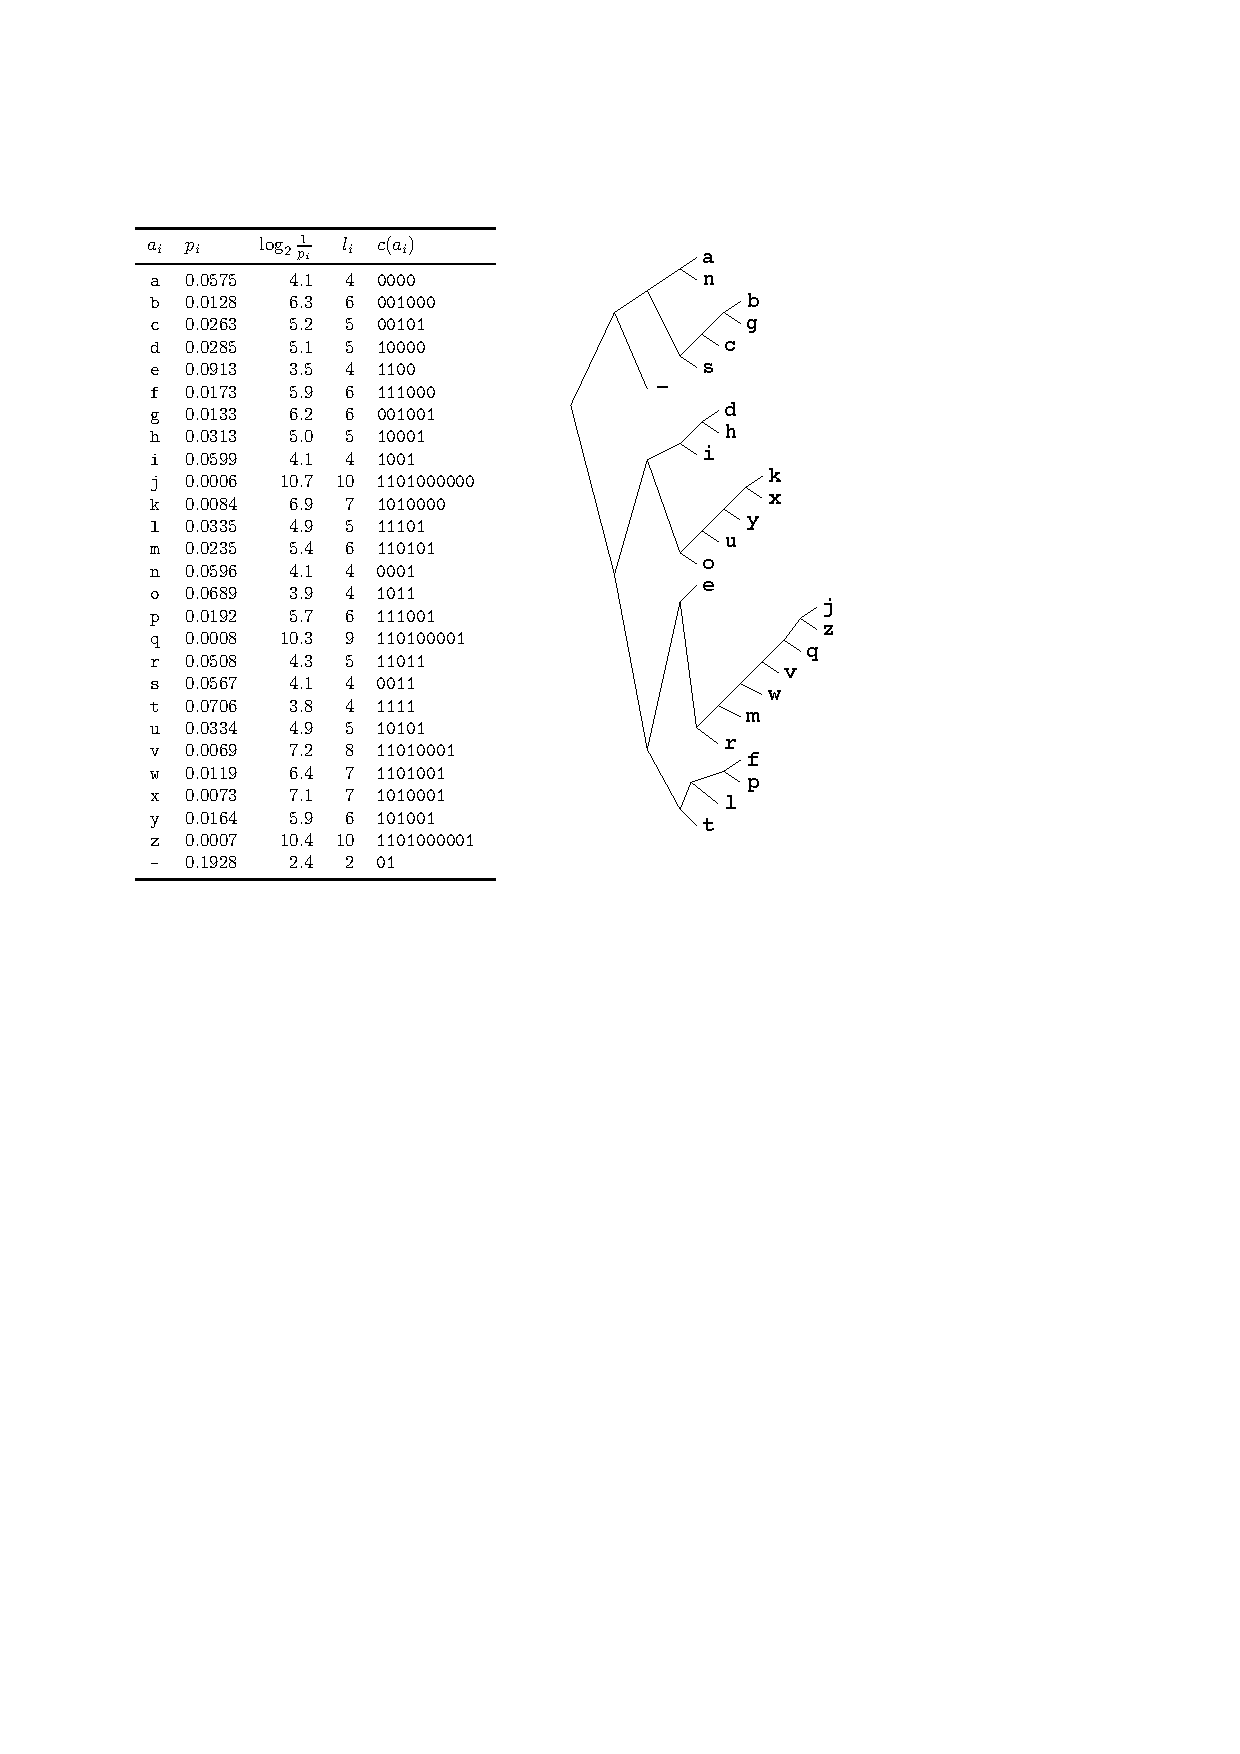
\includegraphics[width=.6\columnwidth]{huffman}
    \end{center}
    \label{fig:huffman}
\end{figure}
Huffman codes are constructed by ``bottom-up'' agglomerative merging of lowest probability symbols. \\ {\tiny Figure from \cite{MacKay2003}}.
}

\subsection{Doing better than Huffman coding}
\frame[t]{
\begin{block}{Drawbacks of Huffman codes}
Only optimal if source is i.i.d. and single symbol transmitted
\begin{itemize}
\item $H(\mathcal{X}) \leq L(C,\mathcal{X}) \leq  H(\mathcal{X}) +1$ bound is {\em per-symbol}
\item $H(\mathcal{X}_2|\mathcal{X}_1) \leq H(\mathcal{X}_2)$, information always reduces entropy.
\item Entire source must be processed to estimate the optimal codebook 
\item Codebook must be transmitted before data -- often highly redundant
\end{itemize}
\end{block}
\begin{block}{Fixes}
\begin{itemize}
\item Code {\em blocks} or ``words'' $\x = [x_1,x_2,\ldots,x_N] \in \Sigma^N$ of the input (trade-off -- requires more complex model)
\item Incrementally build codebook (inefficient, bottom-up)
\item Use {\em arithmetic coding} instead. \end{itemize}
\end{block}
}

\subsection{Compressing `$\mbox{bbba}\square$' using arithmetic coding}
\frame[t]{
Arithmetic coding can be seen as using fractions of bits to encode a symbol.
\begin{figure}[t]
    \begin{center}
        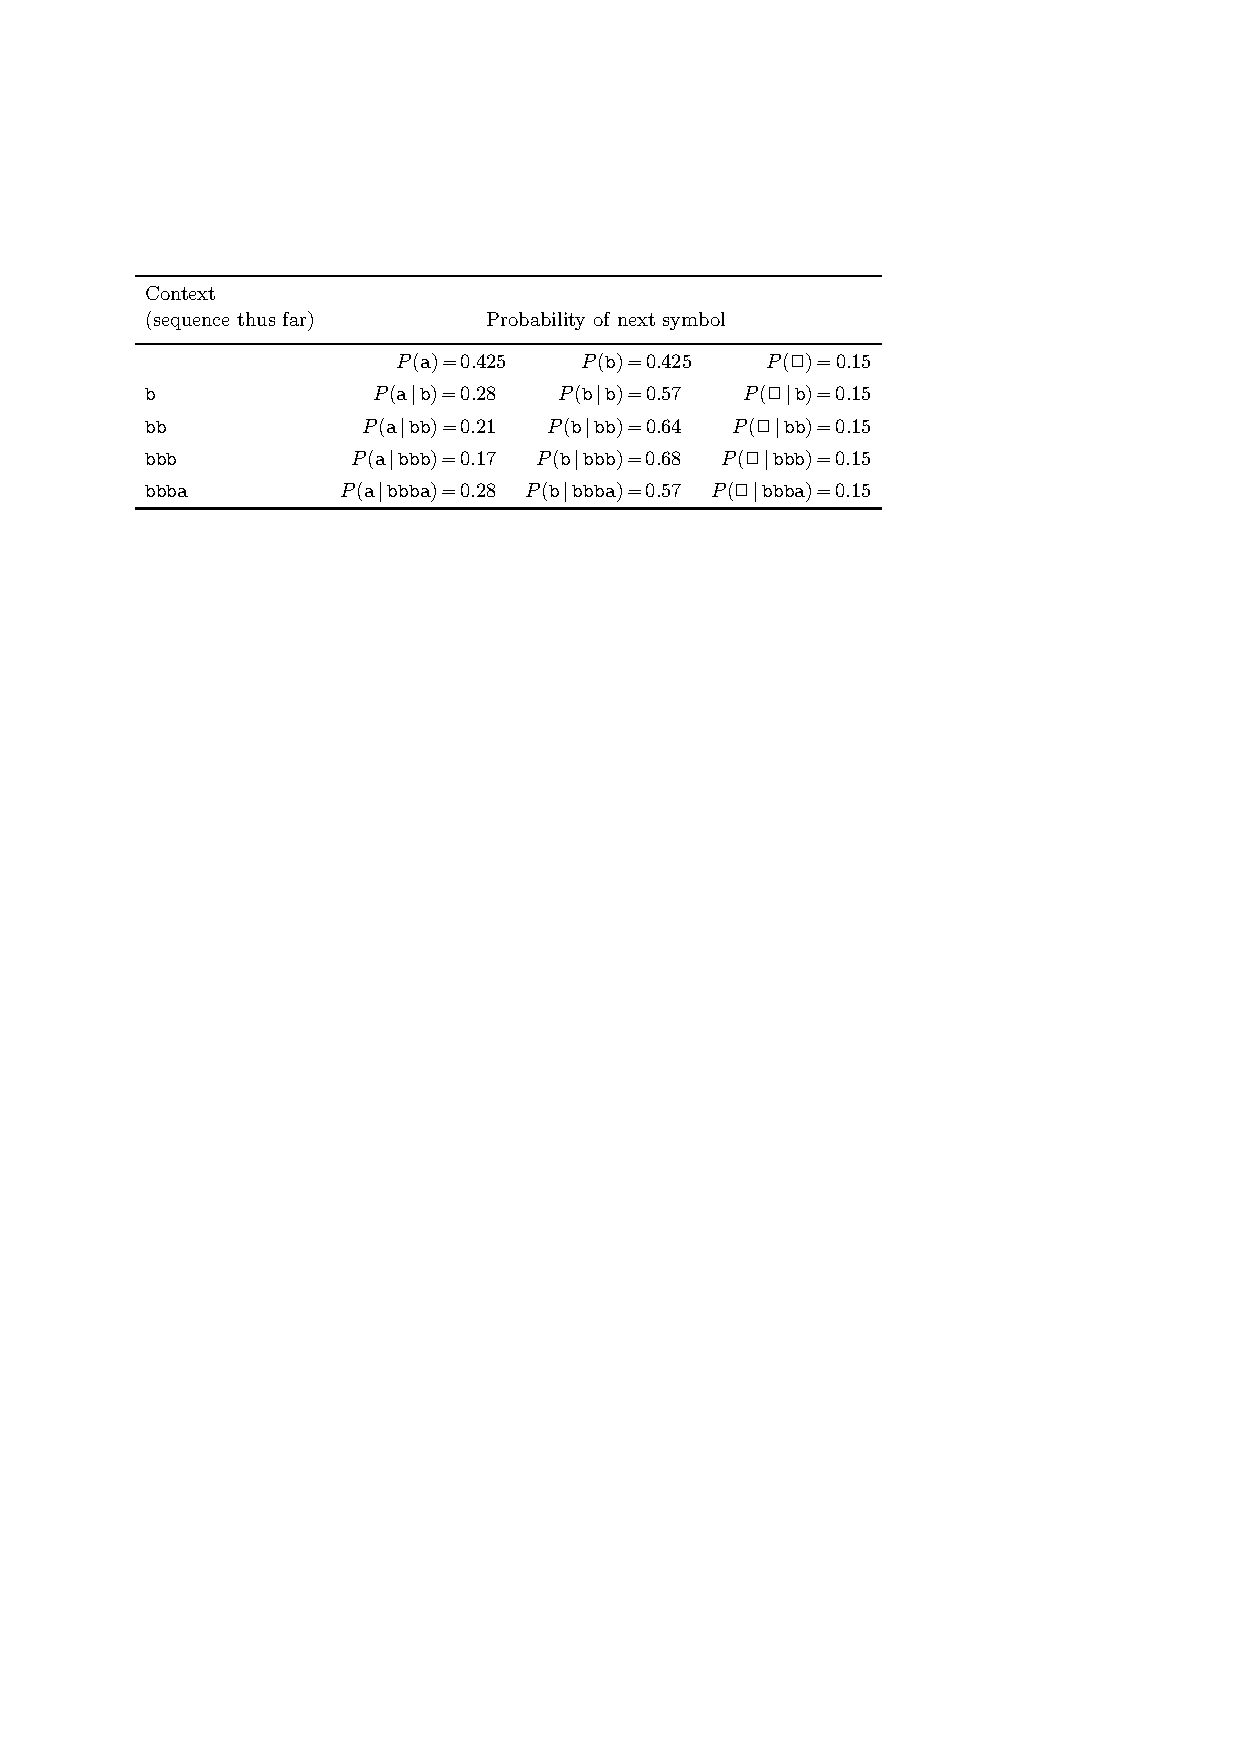
\includegraphics[width=.8\columnwidth]{predictive_probs}\footnote{From \cite{MacKay2003}}
    \end{center}
    \label{fig:predictive_probs}
\end{figure}
Example predictive probabilities over English characters.
}
\frame[t]{

%\begin{pgfpicture}{0cm}{0cm}{5cm}{5cm} 
% (0cm,0cm) is the lower left corner, 
% (5cm,2cm) is the upper right corner. 
%\pgfrect[stroke]{\pgfpoint{0cm}{0cm}}{\pgfpoint{2cm}{10pt}} 
% Paint a rectangle (stroke it, do not fill it)
% The lower left corner is at (0cm,0cm) 
% The rectangle is 2cm wide and 10pt high. 
%\pgfcircle[fill]{\pgfpoint{3cm}{1cm}}{10pt} 
% Paint a filled circle % The center is at (3cm,1cm) % The radius is 10pt
% \end{pgfpicture}

\begin{figure}[t]
    \begin{center}
        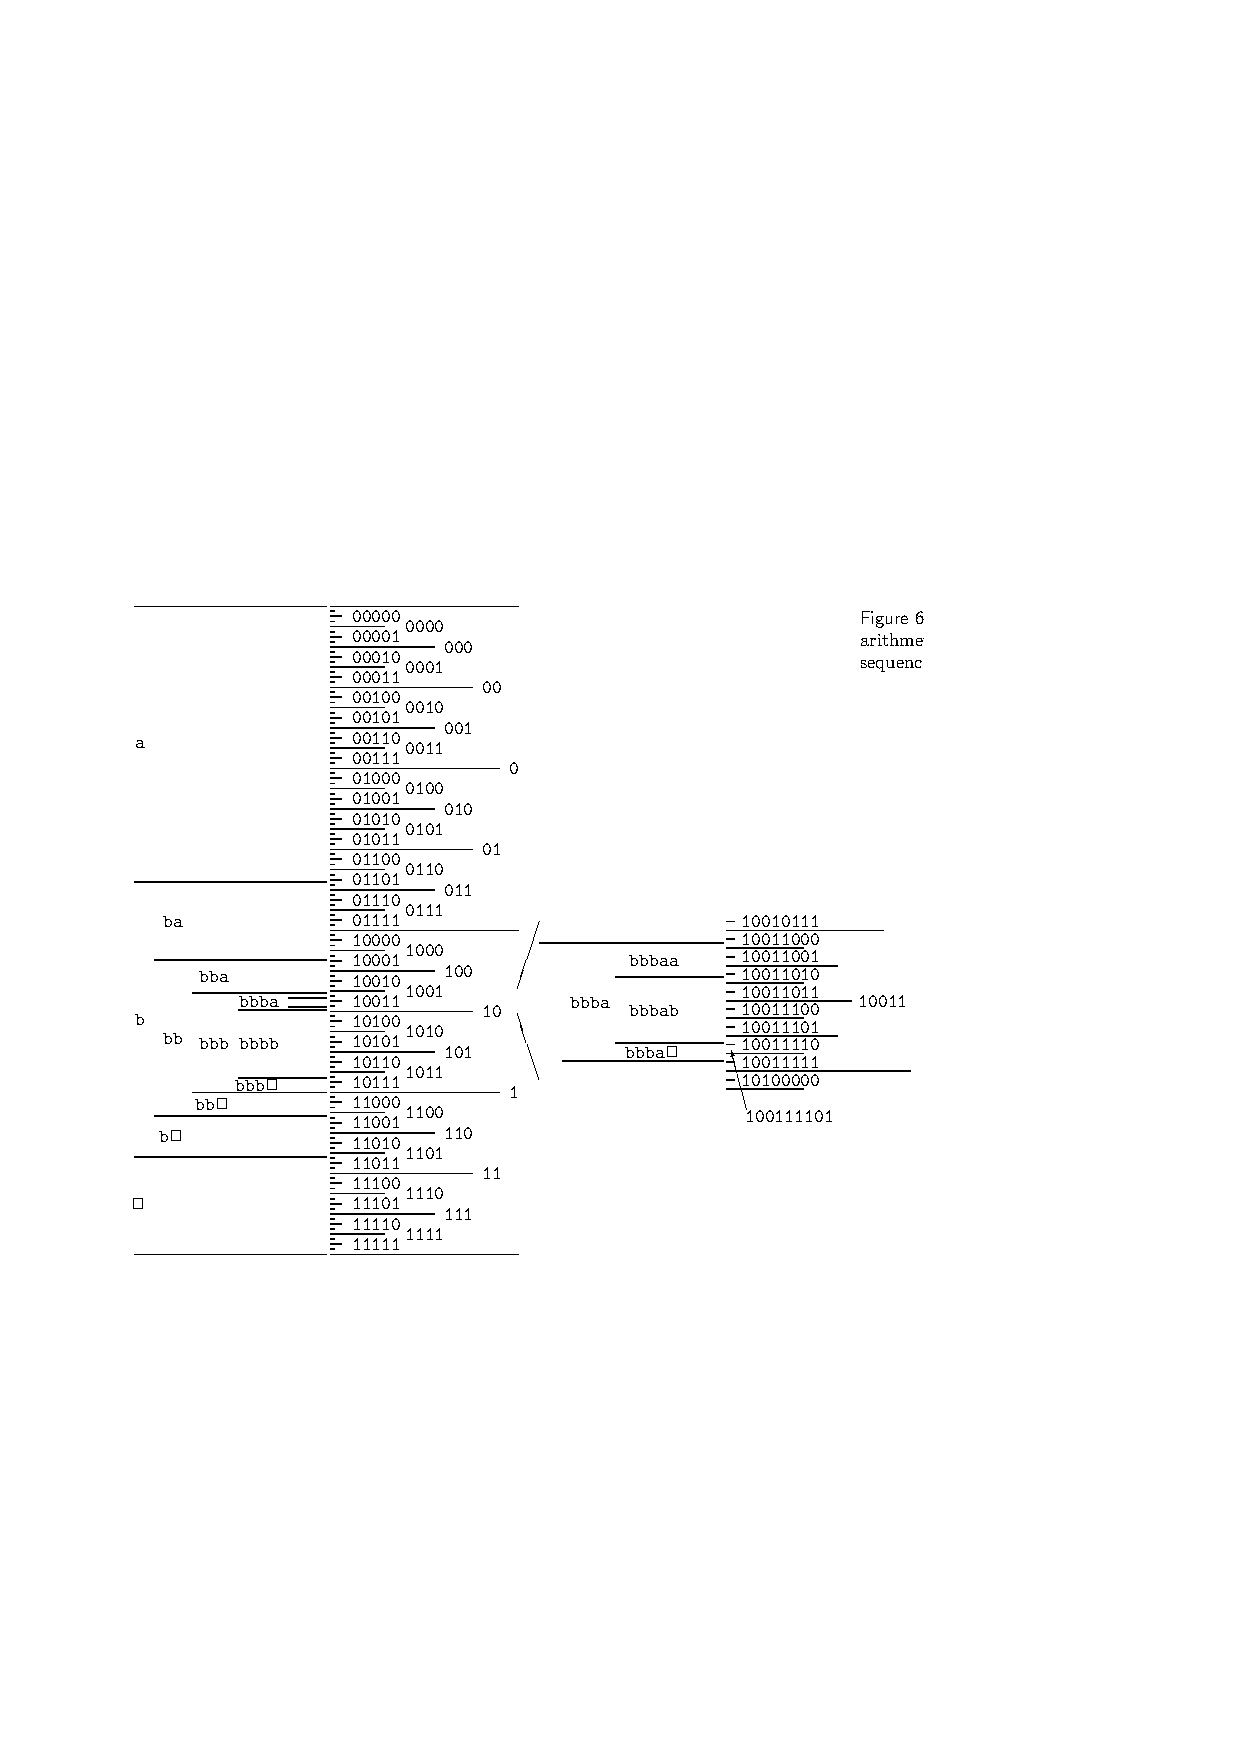
\includegraphics[width=.8\columnwidth]{arithmetic_coding}
        %\pgfsetcolor{fill}{white}
        \pgfrect[fill]{\pgfpoint{-1cm}{5.5cm}}{\pgfpoint{2cm}{2cm}} 
    \end{center}
    \label{fig: arithmetic_coding}
\end{figure}
Schematic of arithmetic coding {\tiny Figure from \cite{MacKay2003}}.


}

\frame[t]{
\begin{block}{Average code length for arithmetic coding \cite{sayood2000}}
If we redefine $X$ to be a R.V. taking values $\x_i \in \Sigma^+$ with probability $P(X=\x_i)$, and consider the ensemble $\mathcal{X} =\{X,\Sigma^+,P\}$ an arithmetic code $C$ has expected length $L(C,\mathcal{X})$ satisfying
\[ H(\mathcal{X}) \leq L(C,\mathcal{X}) \leq  H(\mathcal{X}) +2 \]
\vspace{.5cm}
\end{block}
}

\subsection{Recipe}
\frame[t]{
\begin{block}{Streaming compressor, encoder}
Repeat
\begin{itemize}
\item Compute cumulative predictive distribution $F(x_i|x_{1:(i-1)})$
\item Send CDF boundary for $x_i$ to arithmetic encoder
\item Update model to include $x_i$ in {\em context} $x_{1:(i-1)}$
\end{itemize}
\end{block}


\begin{block}{Streaming compressor, decoder}
Repeat
\begin{itemize}
\item Compute cumulative predictive distribution $F(x_i|x_{1:(i-1)})$
\item Process bits until CDF interval distinct
\item Conclude $x_i$ sent from encoder
\item Update model to include $x_i$ in {\em context} $x_{1:(i-1)}$
\end{itemize}

\end{block}
}

\subsection{Streaming compression requirements}
\begin{frame}[t]{}
Predictive model
\begin{itemize}
\item Incremental estimator for all conditional distributions given a single observation sequence of unbounded length
\item Estimator must have worst case linear time complexity.
%\begin{itemize}
%\item Joint because we want all marginal and conditional distributions
%\item Single observation because we only see a single data ``stream.''
%\end{itemize}
\item The model must be representable in worst case constant space.
\item Predictive inference must be performed in worst case constant time.
\end{itemize}

%\begin{alertblock}{Nature of Problems}
%Computational
%\end{alertblock}
\end{frame}	

\subsection{Compression as testbed}
\begin{frame}[t]{}
\begin{itemize}
\item Comparison between probabilistic and deterministic models possible.
\item Better compression and better modeling intimately related.
\item Performance measured in {\em bits}, {\em log-loss} (bits per byte), or {\em perplexity} instead of likelihood or evidence.
\end{itemize}

%\begin{alertblock}{Nature of Problems}
%Computational
%\end{alertblock}
\end{frame}	

\section{Intuition}
%\section[Outline]{}
%\frame[t]{\tableofcontents}
\subsection{Sequence of discrete observations from an arbitrary stochastic process}
\frame[t]{
\begin{block}{Binary sequence (model definitions)}
\[
\begin{array}{l}
0,1,0,0,1,0,0,1...
\end{array}
\]
\end{block}
%\frametitle{Sequential Discrete Observations}
\begin{block}{Byte sequence  (compression experiments)}
\[
\begin{array}{l}
01001001 , 01101110 , 00100000 , 01110100,\\
01101000 , 01110010 , 01100101 , 01100101,\\
%00100000 , 01100100 , 01100001 , 01111001,\\
%01110011 , 00100000 , 01111001 , 01101111,\\
%01110101 , 01110010 , 00100000 , 01101000,\\
%01100001 , 01110010 , 01100100 , 00100000,\\
%01100100 , 01110010 , 01101001 , 01110110,\\
%01100101 , 00100000 , 01110111 , 01101001,\\
01101100 , 01101100 , 00100000 , 01100011,\\
01110010 , 01100001 , 01110011 , 01101000\ldots
\end{array}
\]
\end{block}

\begin{block}{Abitrary-ary sequence (language modeling future work)}
\[
\begin{array}{l}
0101 , 0110111000100000 , 00100,\\
00 , 01110 , 011001001100101,\\
%00100000 , 01100100 , 01100001 , 01111001,\\
%01110011 , 00100000 , 01111001 , 01101111,\\
%01110101 , 01110010 , 00100000 , 01101000,\\
%01100001 , 01110010 , 01100100 , 00100000,\\
%01100100 , 01110010 , 01101001 , 01110110,\\
%01100101 , 00100000 , 01110111 , 01101001,\\
%01101100 , 01101100 , 00100000 , 01100011,\\
01110010 01100001 01110011, 1\ldots
\end{array}
\]
\end{block}

}



\subsection{General-purpose predictive model desiderata and assumptions}
\begin{frame}[t]{}
Desiderata
\begin{itemize}
\item Incrementally estimate a large set of (or all) conditional distributions in worst case time linear in the length of an unbounded sequence of observations.
%\begin{itemize}
%\item Joint because we want all marginal and conditional distributions
%\item Single observation because we only see a single data ``stream.''
%\end{itemize}
\item Represent the model in worst case constant space.
\item Do predictive inference in worst case constant time.
\end{itemize}
Assumptions
\begin{itemize}
\item Shortness is good
\item Recency matters
\item Power-laws permeate
%\begin{itemize}
\end{itemize}
%\begin{alertblock}{Nature of Problems}
%Computational
%\end{alertblock}
\end{frame}	

\subsection{Notation, fixed Markov model}
\begin{frame}[t]{}
Let $\Sigma$ be a set of symbols, let $\x = x_1, x_2, ..., x_T$ be an observed sequence with $x_t \in \Sigma$.  Also let $s,s' \in \Sigma$ and $\context \in \Sigma^+$.  Then
\begin{align*}
G_\context(s)=\frac{N(\context s)}{\sum_{s'\in\Sigma}N(\context s')}\label{eqn:mll}
\end{align*}
is the maximum likelihood estimator for the conditional distribution ${\hat P}(X=s|\context) \equiv G_\context(s)$.
\vspace{.5cm}

Estimating a finite set of conditional distributions corresponding to a finite set of ``contexts'' or ``states'' $\context$ generally yields a {\em bad} model.

\vspace{.5cm}
Why bad?  Long $\context$.  Maximum likelihood overconfident.

\vspace{.5cm}
Note: first stochastic memoization rule.  Only those $s$'s seen before returned.

\end{frame}	

\subsection{An aside: stochastic memoization}
\begin{frame}[t]{}
A stochastic memoizer \cite{Goodman2008} is a non-deterministic function cache 
\begin{align*}
SM(\context) = \left\{\begin{array}{ccc}
\sigma_1  & \mbox{w.p.}  &  G_\context(\sigma_1) \\
\sigma_2  & \mbox{w.p.}  &  G_\context(\sigma_2)  \\
  &  \vdots &   
\end{array}\right.
\end{align*}
with $\sigma_i \in \Sigma$.
\vspace{.5cm}

Posterior inference in many Bayesian nonparametric models can be described in terms of stochastic memoization. 
\end{frame}

\subsection{Bayesian approach}
\begin{frame}[t]{}
Can treat $G$'s as random and integrate them out like
\begin{align*}
P(x_{T+1}=s|\data) = \int P(x_{T+1}=s|G)P(G|\data)dG = {\EE[G(s)] } ,
\end{align*}
yielding, for instance,
\begin{align*}
\EE[G_\context(s)]=\frac{N(\context s) + \frac{\alpha}{|\Sigma|}}{\sum_{s'\in\Sigma}N(\context s') + \alpha}
\end{align*}
in the case of independent Dirichlet priors, i.e.~$G_\context \sim \Dir(\frac{\alpha}{|\Sigma|})$

\vspace{.5cm}
The prior makes the estimate more conservative.  Can do better by sharing statistical strength.

\vspace{.5cm}
Note: new stochastic memoization rule.  Unobserved $\sigma$'s can be returned.  Good values of $\alpha$ can improve predictive performance.

\end{frame}

\subsection{Hierarchical Bayesian approach (i.e.~Hierchical Dirichlet Process (HDP) \cite{Teh2006b})}
  \frame[t] {%slide 9
Can relate $G_\context$ to related distribution $G_\parent$ where, for instance, $\sigma(x_1x_2x_3\ldots x_n) = x_2x_3\ldots x_n$ could be the suffix operator
\[\EE[\G_\context(s)]
= \EE\left[
\frac{N(\context s)+ \alpha \G_\parent(s)}{\sum_{s'\in\Sigma} N(\context s') + \alpha}\right]
\]
Where now the counts
\[\{N(\ubf's')\}_{\ubf'\in\Sigma^+, s'\in\Sigma}\], along with $\alpha$, must be averaged over, typically using Monte Carlo methods.

\vspace{.5cm}
Note: stochastic memoizer now can return unobserved $\sigma$'s in the context $\context$ {\em and} the probability of returning any given symbol is affected by the probability of it being returned by other, related contexts.
}






 %for DP's and PYP's we will sample directly from $P(x_{i+1} | \xbf_{1:i})$ given a marginalized representation of the hierarchy $\GG$ consisting of counts 
 %\[P(x_{i+1} | \xbf_{1:i}) \approx \frac{1}{L}\sum_{\ell = 1}^L P(x_{i+1} | \xbf_{1:i}, \GG_\ell), \; \GG_\ell \sim P(\GG | \xbf_{1:i})\]

 

 % \frame[t] {%slide 9
%\begin{align}
%\label{eq:predictive}
%P(x_{T+1}=s|\data) = \int P(x_{T+1}=s|G)P(G|\data)dG = {\EE[G(s)] } ,
%\end{align}
% }




\section{Models}



\subsection{Sequence Memoizer}

\frame[t] {
\begin{block}{Sequence memoizer (SM), \citet{Wood2011}}
The SM is a compactly-representable, unbounded-depth, hierarchical, Bayesian-nonparametric prior over discrete sequence distributions for which incremental Bayesian updating and predictive inference is efficient.
\end{block}
}

 \subsection{Notation}
 \frame[t] {%slide 8
 Let $\GG = \{\G_{\context}\}, \forall \context \in \Sigma^+$ be {\em all} conditional distributions over a countable alphabet $\Sigma$ and $\xbf = x_1, x_2, \ldots, x_i, \ldots \in \Sigma^+$ be a sequence of discrete observations. The joint distribution of $\xbf$ and $\GG$ is
\begin{eqnarray*}
P(\xbf,\GG) &=& P(\GG)P(\xbf|\GG) \nonumber \\
P(\xbf,\GG) &=& P(\GG)\prod_{i=0}^{|\xbf|-1}G_{\xbf_{1:i}}(\xbf_{i+1})
\end{eqnarray*}
Expanding $P(\xbf|\GG)$ makes this clearer,
\begin{align}
P(\xbf|\GG) = G_{\varepsilon}(x_{1})G_{x_1}(x_{2})G_{\xbf_{1:2}}(x_{3})\cdots G_{\xbf_{1:(|\xbf|-1)}}(x_{|\xbf|})  \nonumber 
\end{align}
Note that this is the joint\footnote{$P(x_1,\ldots,x_i|\theta) = P(x_1|\theta) P(x_2 | x_1, \theta) P(x_3 | x_1,x_2, \theta) \cdots P(x_i | \xbf_{1:(i-1)}, \theta)$} distribution of $\xbf$. The prior $P(\GG)$ directly regularizes the joint distribution itself.
 }



 \subsection{Inference sketch}
  \frame[t] {%slide 9
Bayesian inference
\begin{itemize}
\item Prediction
 \[P(x_{i+1}=s | \xbf_{1:i}) = \int P(x_{i+1}=s | \GG) dP(\GG | \xbf_{1:i}) = \EE[\G_\context(s)] \]
\item Posterior updating (sketch)
\[P(\GG|\data_{1:i}) \propto P(x_i | \GG) P(\GG | \data_{1:(i-1)})\]

\end{itemize}
where $\context = \xbf_{1:i}$.
}



\subsection{(Binary) sequence memoizer = (binary) hierarchical PY process \cite{Teh2006a} of unbounded depth.}

  \frame[t] {%slide 27
 %\frametitle{A Way to Tie Together ``Related'' Conditional Distributions}
 \begin{figure}[htbp]
\begin{center}
%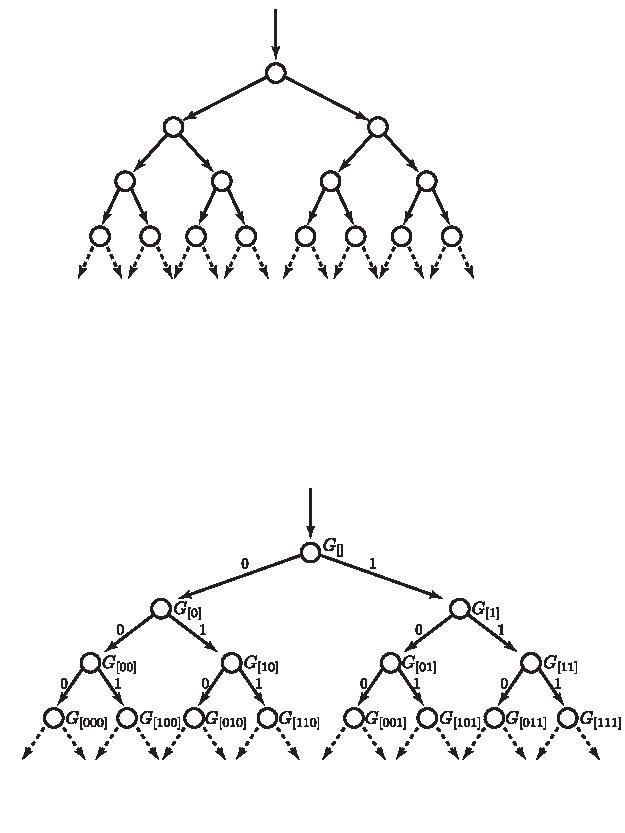
\includegraphics[trim = 4cm 8cm 4cm 8cm, clip, width=5cm]{jtfig/base.pdf}
\vspace{2cm}
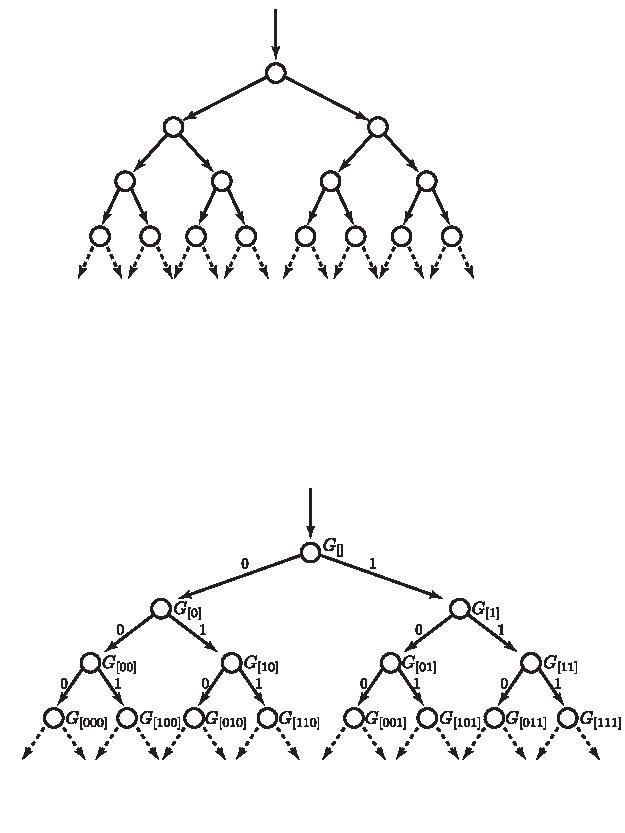
\includegraphics[trim = 2cm 2cm 2cm 10cm, width=8cm]{jtfig/base.pdf}
%\caption{Test perplexity vs.~number of training observations.}
\label{fig: gm_binary_complete}
\end{center}
\end{figure}
}

\subsection{Pitman-Yor process}
\frame[t] {
%\frametitle{Pitman Yor Process (PYP) : Definition \cite{Pitman1997a}}
 A Pitman-Yor process $\PY(c,d,H)$ is a distribution over distributions with three parameters
\begin{itemize}
\item A discount $ 0 \le d < 1 $ that controls power-law behavior
\begin{itemize}
\item $d=0$ is Dirichlet process (DP)
\end{itemize}
\item A concentration $c > -d$ like that of the DP
\item A base distribution $H$ also like that of the DP
\end{itemize}
\vspace{.25cm}
Key properties (more to come): \newline

If $G\sim\PY(c,d,H)$ then {\em a priori}

\begin{itemize}
\item $\EE[G(s)] = H(s)$
\item $\Var[G(s)] = (1-d)H(s)(1-H(s))$
\end{itemize}

}

\subsection{Binary sequence memoizer notation}
  \frame[t] {%slide 27
  Example
% \frametitle{Sequence Memoizer, \citet{Wood2009}}
\begin{eqnarray*}
\Sigma &=& \{0,1\}\\
\U_{\Sigma } &=& [.5, .5] \\
\\
	\G_{\varepsilon} | \U_{\Sigma}, d_0 &\sim& \PY(d_0, 0, \U_{\Sigma }) \\
		\G_{\bf{u}} | \G_{\sigma(\bf{u})}, d_{|\bf{u}|} &\sim& \PY(d_{|\bf{u}|}, 0, \G_{\sigma(\bf{u})}) \hspace{.35cm} \forall {\bf u} \in \Sigma^+\\
	x_n | x_1,  \ldots, x_{n-1} = \bf{u} &\sim& \G_{\bf{u}}
\end{eqnarray*}
Here $\sigma(x_1x_2x_3\ldots x_n) = x_2x_3\ldots x_n$ is the suffix operator.
\bigskip

\begin{itemize}
\item Recency effects are encoded by coupling related conditional distributions (``back-off'')
\item Power-law effects are encoded by the choice of hierarchical modeling glue: the Pitman-Yor process (PY).
\end{itemize}


}

% \frame[t] {%slide 27
% \frametitle{Sequence Memoizer, \citet{Wood2009}}

%\begin{align}
%\prob_\varepsilon &\sim \py(\disc_0,\prob_0)  \label{eqn:hierbayes}\\
%\prob_\context|\prob_\parent &\sim \py(\disc_{|\context|},\prob_\parent) &&
%\text{for all $\context\in\Sigma^{*}_n\backslash\varepsilon$} \nonumber\\
%x_i|\mathbf{x}_{i-n:i-1}=\context,\prob_\context &\sim \prob_\context &&
%\text{for $i=1,\ldots,T$}  \nonumber
%\end{align}
%}


\subsection{Linear space sequence memoizer, \citet{Wood2009}}
\begin{frame}[t] \frametitle{}
PY properties used to achieve linear space sequence memoizer.
\begin{columns}[c] \column{.5\textwidth} 
\begin{block}{Coagulation \cite{Pitman1999, Ho2006}}
If \[G_2| G_1\sim\py(d_1,0,G_1)\] and \[G_3| G_2\sim\py(d_2,0,G_2)\] then
\[G_3|G_1\sim\py(d_1d_2,0,G_1)\] with $G_2$ marginalized out.
\label{thm:coag}
\end{block}
\column{.5\textwidth} 
\begin{block}{Fragmentation \cite{Pitman1999, Ho2006,Wood2009}}
Suppose
 \[G_3| G_1\sim\py(d_1d_2,0,G_2)\]
 then $G_3$
 can be ``fragmented'' so 
 \[G_2 | G_1 \sim \py(d_1,0,G_1)\]
 and
  \[G_3| G_2\sim\py(d_2,0,G_2)\] 
  if $G_2$ is needed.
\end{block}
 \end{columns}
 \end{frame}



\comment{
  \frame[t] {%slide 27
 \frametitle{Graphical Model for 110100}
 \begin{figure}[htbp]
\begin{center}
%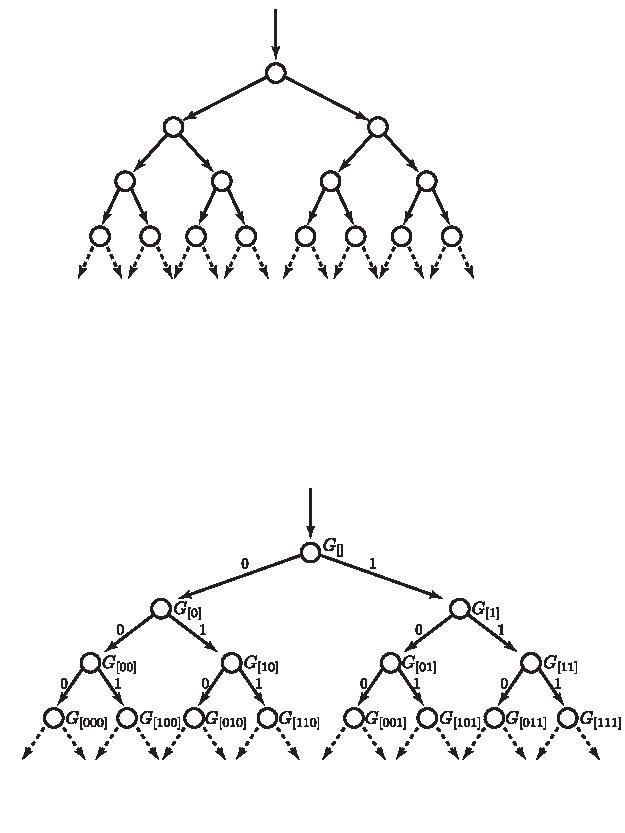
\includegraphics[trim = 4cm 8cm 4cm 8cm, clip, width=5cm]{jtfig/base.pdf}
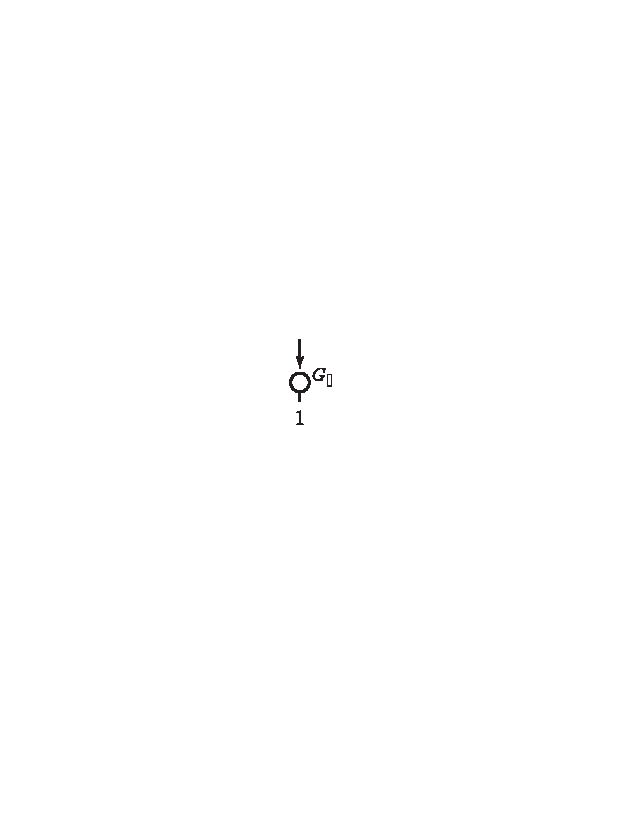
\includegraphics[trim = 2cm 2cm 2cm 6cm, width=8cm]{jtfig/seq_1.pdf}
%\caption{Test perplexity vs.~number of training observations.}
\label{fig: gm_binary_complete}
\end{center}
\end{figure}

 }
 
   \frame[t] {%slide 27
 \frametitle{Graphical Model for 110100}
 \begin{figure}[htbp]
\begin{center}
%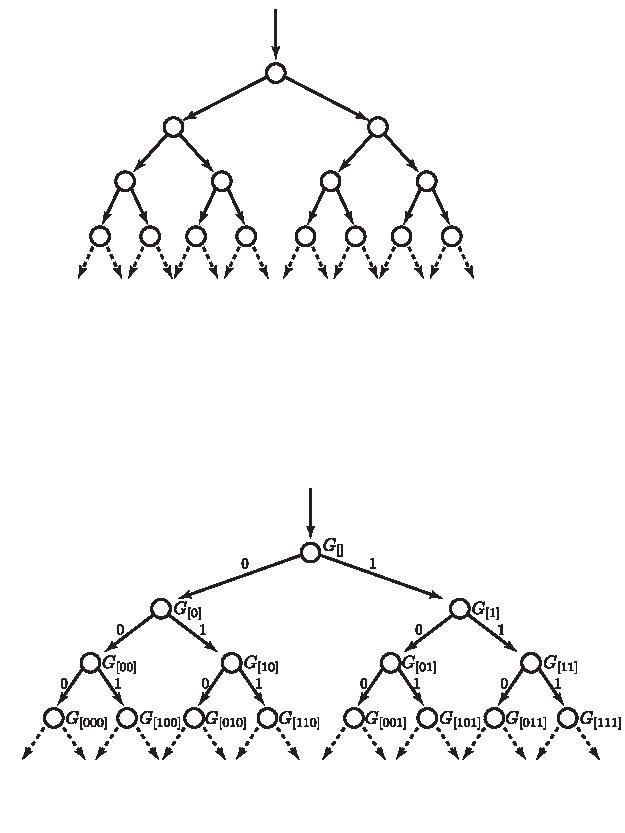
\includegraphics[trim = 4cm 8cm 4cm 8cm, clip, width=5cm]{jtfig/base.pdf}
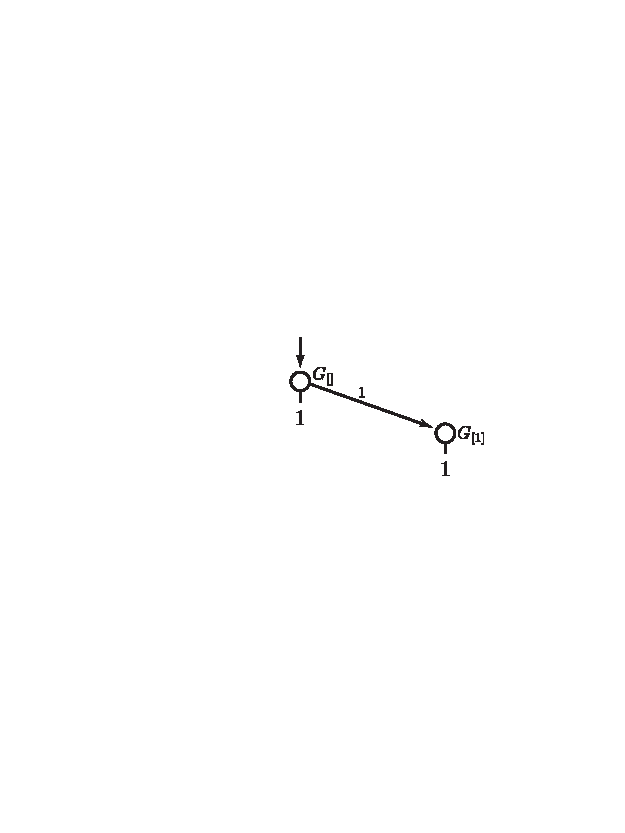
\includegraphics[trim = 2cm 2cm 2cm 6cm, width=8cm]{jtfig/seq_2.pdf}
%\caption{Test perplexity vs.~number of training observations.}
\label{fig: gm_binary_complete}
\end{center}
\end{figure}

 }

  \frame[t] {%slide 27
 \frametitle{Graphical Model for 110100}
 \begin{figure}[htbp]
\begin{center}
%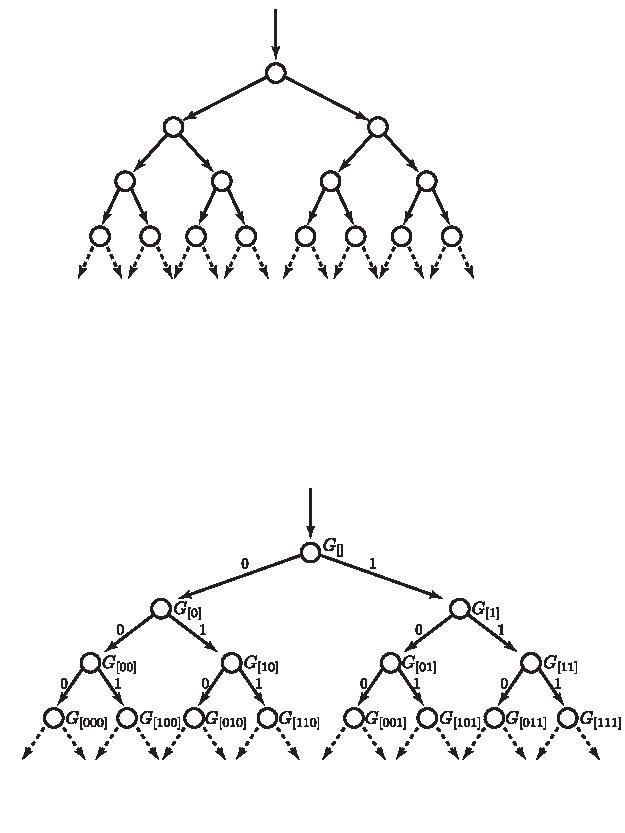
\includegraphics[trim = 4cm 8cm 4cm 8cm, clip, width=5cm]{jtfig/base.pdf}
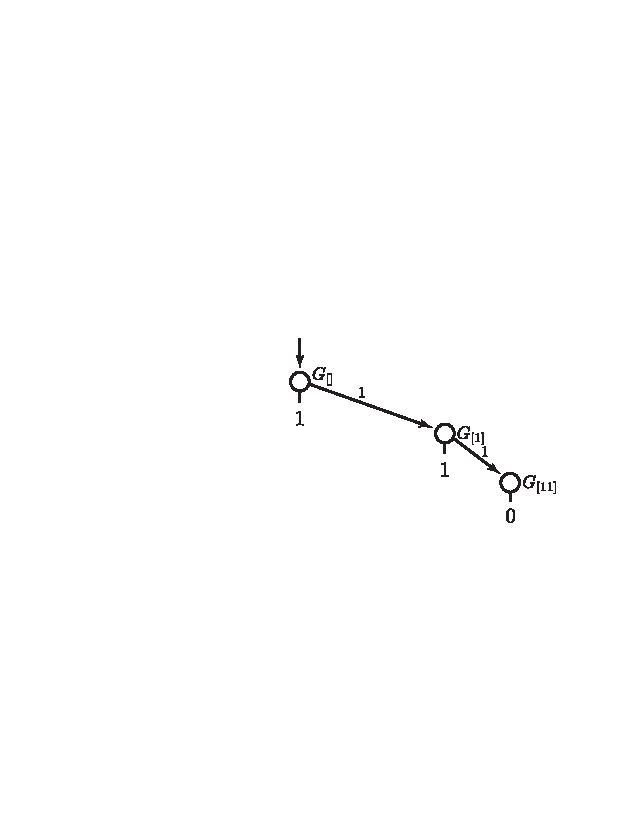
\includegraphics[trim = 2cm 2cm 2cm 6cm, width=8cm]{jtfig/seq_3.pdf}
%\caption{Test perplexity vs.~number of training observations.}
\label{fig: gm_binary_complete}
\end{center}
\end{figure}

 }
   \frame[t] {%slide 27
 \frametitle{Graphical Model for 110100}
 \begin{figure}[htbp]
\begin{center}
%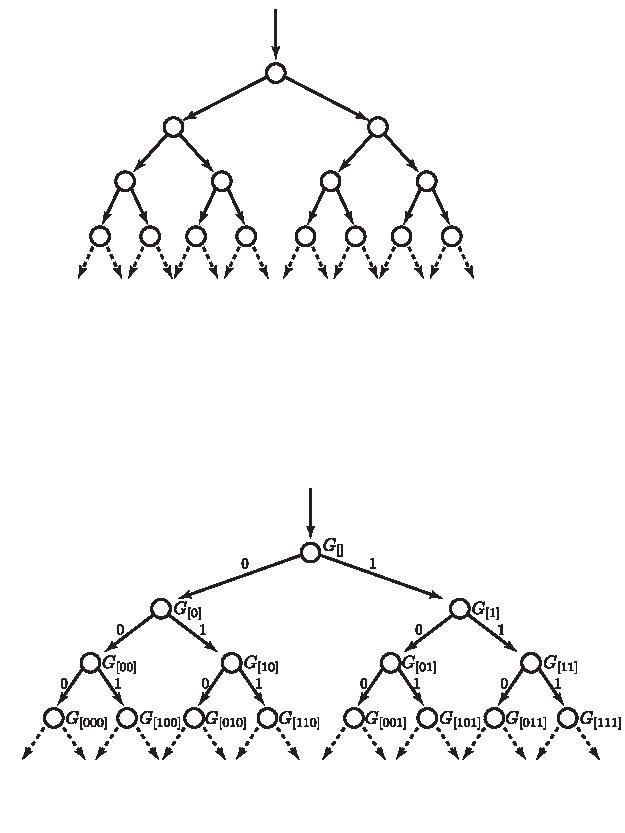
\includegraphics[trim = 4cm 8cm 4cm 8cm, clip, width=5cm]{jtfig/base.pdf}
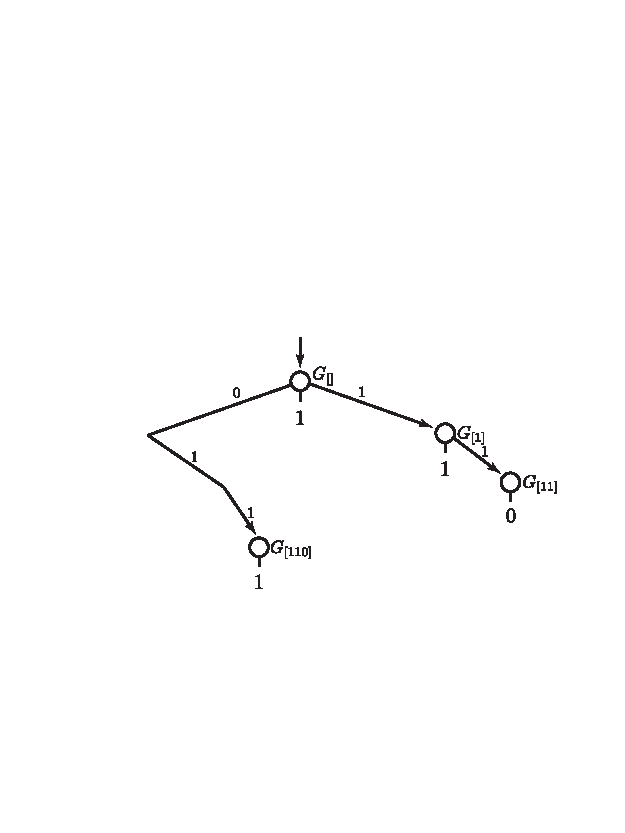
\includegraphics[trim = 2cm 2cm 2cm 6cm, width=8cm]{jtfig/seq_4.pdf}
%\caption{Test perplexity vs.~number of training observations.}
\label{fig: gm_binary_complete}
\end{center}
\end{figure}

 }
   \frame[t] {%slide 27
 \frametitle{Graphical Model for 110100}
 \begin{figure}[htbp]
\begin{center}
%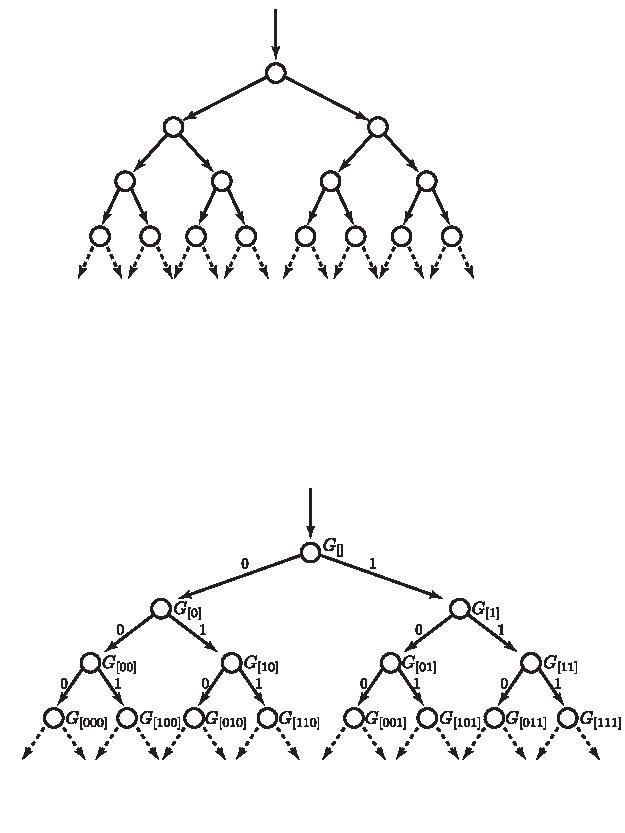
\includegraphics[trim = 4cm 8cm 4cm 8cm, clip, width=5cm]{jtfig/base.pdf}
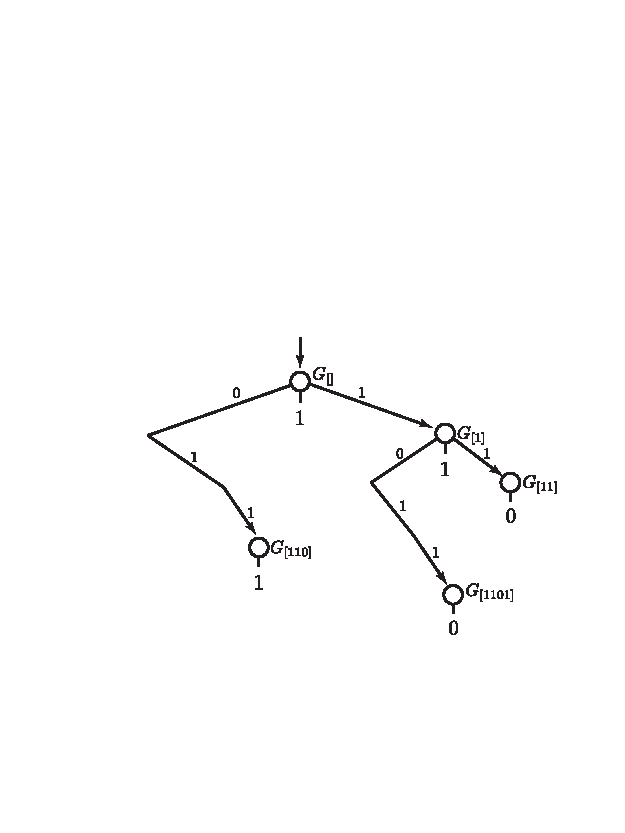
\includegraphics[trim = 2cm 2cm 2cm 6cm, width=8cm]{jtfig/seq_5.pdf}
%\caption{Test perplexity vs.~number of training observations.}
\label{fig: gm_binary_complete}
\end{center}
\end{figure}

 }
 }
 
  \subsection{Resulting binary sequence memoizer for observed sequence 110100}
   \frame[t] {%slide 27
 \begin{figure}[htbp]
\begin{center}
%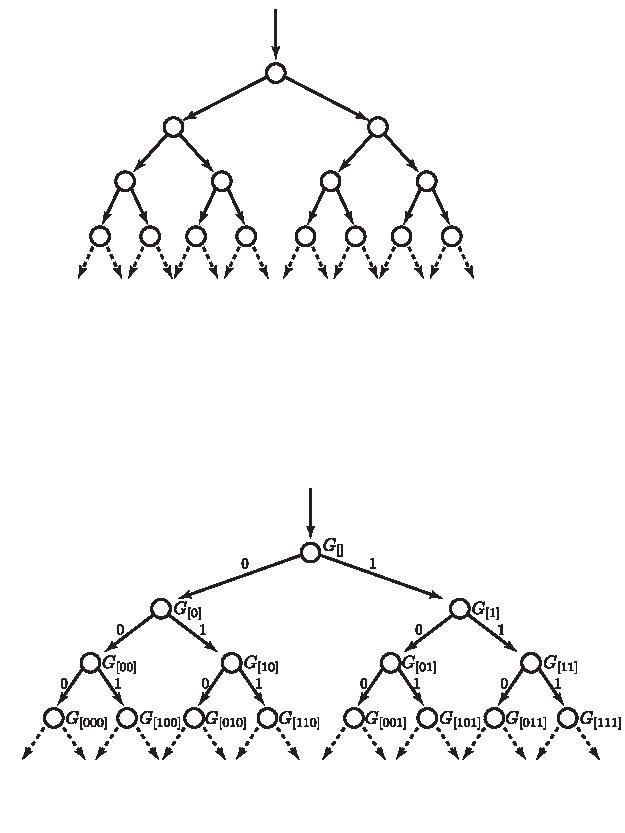
\includegraphics[trim = 4cm 8cm 4cm 8cm, clip, width=5cm]{jtfig/base.pdf}
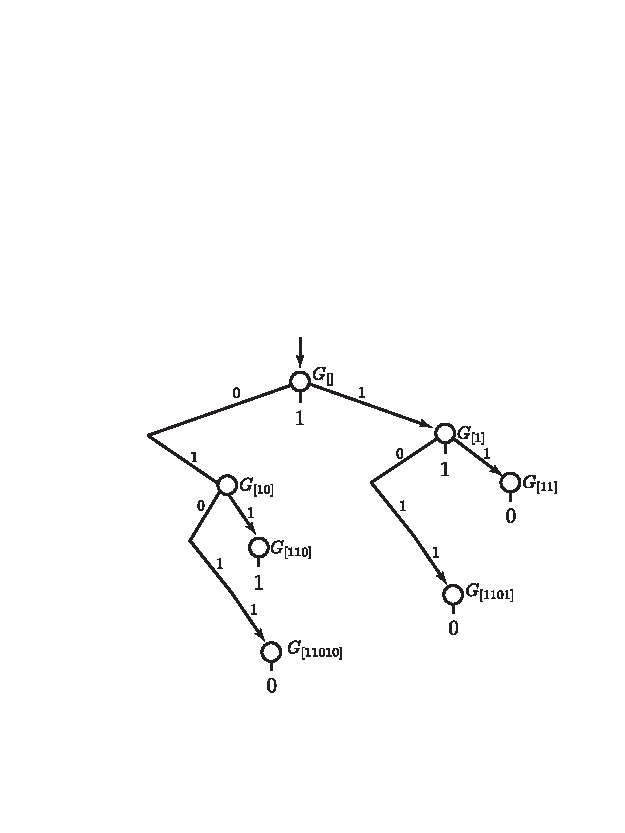
\includegraphics[trim = 2cm 2cm 2cm 6cm, width=8cm]{jtfig/seq_6.pdf}
%\caption{Test perplexity vs.~number of training observations.}
\label{fig: gm_binary_complete}
\end{center}
\end{figure}

 }



\subsection{Inference in the sequence memoizer}
  \frame[t] {%slide 9
\[\EE[\G_\context(s)]
= \EE\left[
\frac{N(\context s)-\disc_{\context} M(\context s) + \left(\disc_{\context}\sum_{s'\in\Sigma}  M(\context s')\right) \G_\parent(s)}{\sum_{s'\in\Sigma} N(\context s')}\right]
\]
is an expectation over a set of random counts (latent variables)
\[\{N(\ubf's'),M(\ubf's')\}_{\ubf'\in\cctx, s'\in\Sigma}\]
which have properties 
\begin{itemize}
\item  $N(\data_{1:i}x_{i+1}) \geq 1 \; \forall \; i$, observations
\item $M(\ubf's') \leq N(\ubf's')$, ``discounting''
\end{itemize}
\vspace{.5cm}
The random count/latent variables are averaged over using Monte Carlo methods.
}


\begin{frame}[t]{}
Posterior inference in the sequence memoizer is hierarchical stochastic memoization of sequence continuations. 
\begin{align*}
SM(\context) = \left\{\begin{array}{ccc}
\sigma_1  & \mbox{w.p.}  &  \EE[G_\context(\sigma_1)] \\
\sigma_2  & \mbox{w.p.}  &  \EE[G_\context(\sigma_2)]  \\
  &  \vdots &   
\end{array}\right.
\end{align*}
with $\sigma_i \in \Sigma$.
\vspace{.5cm}
\end{frame}

\section{Literature}
\subsection{Incremental Estimation}
\begin{frame}[t]{}
First incremental estimation \citet{Gasthaus2010}.  1-PF and Kneser-Ney variant approximately equal.
First scalability to 100's MB's (Wikipedia 1.66 bits/byte, 100MB -> 20.8MB, outperformed by PAQ)
4.35 bits per Chinese character (better than best reported result of 5.44 bits \cite{Wu2007}).
\end{frame}

\subsection{Constant space approximate inference}
\begin{frame}[t]{}
\begin{block}{``Forgetting counts'' \citet{Bartlett2010}}
\begin{figure}[htbp]
\begin{center}
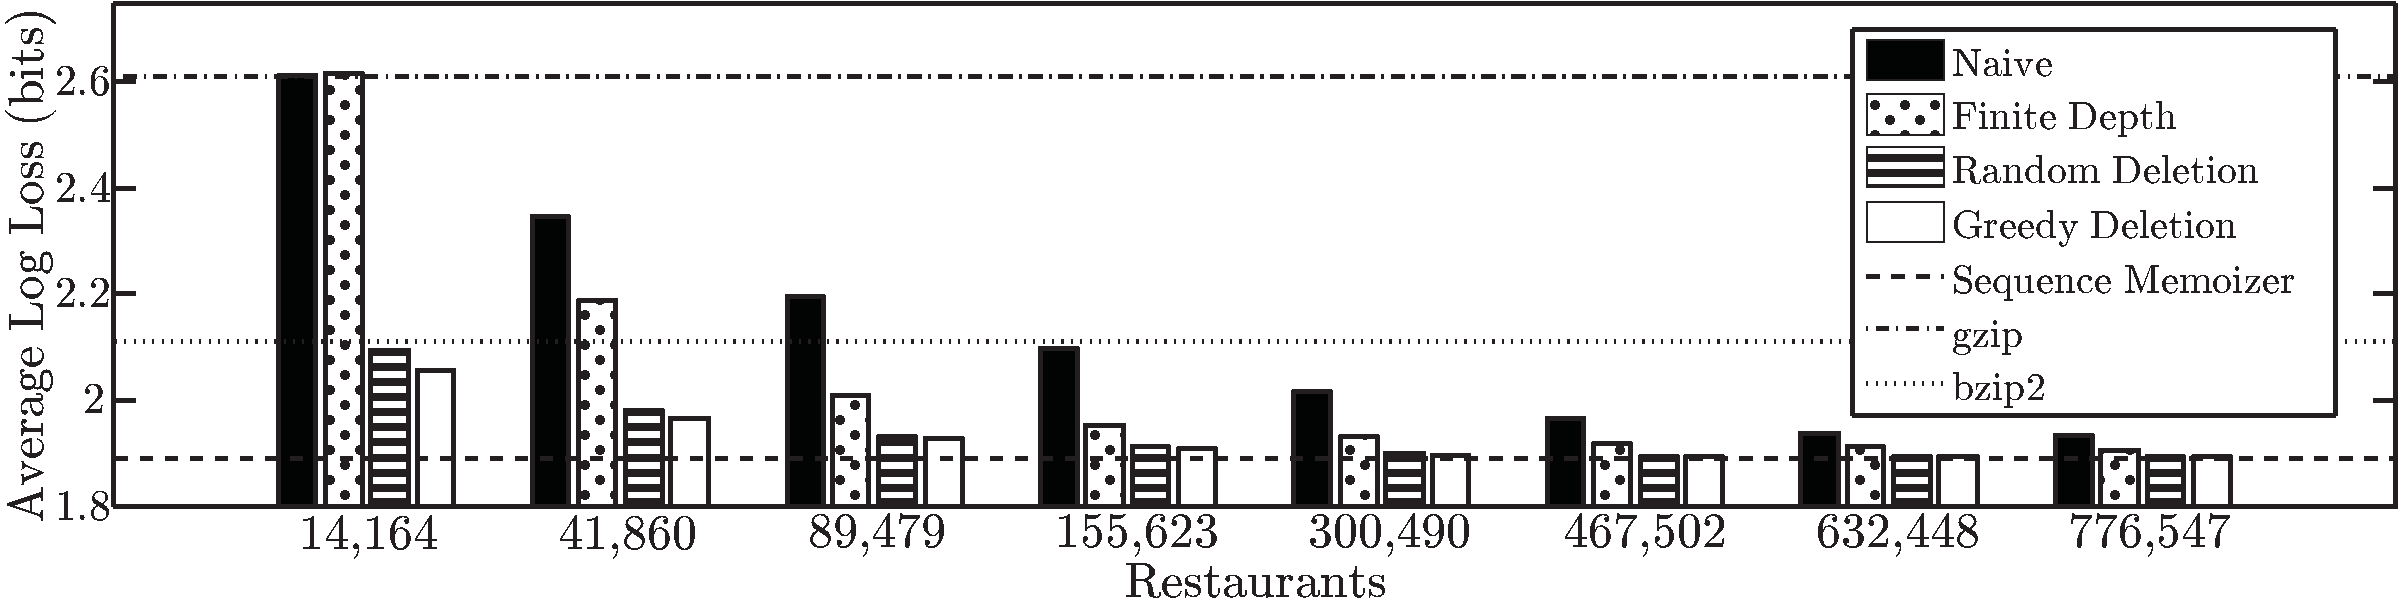
\includegraphics[width=\textwidth]{results_calgary_corpus.pdf}
\end{center}
\end{figure}
A dependent HPYP can be defined though a graphical model leaf node deletion scheme.  Inference in the resulting model was shown to approximate the SM well.  \tiny{data: Calgary corpus, rests = total used nodes in 3-10 grams}
\end{block}
\begin{block}{``Improvements to the sequence memoizer'' \citet{Gasthaus2011}}
Only $O(2|\Sigma|)$ numbers need be stored for each node in the SM graphical model.
\end{block}

\end{frame}

\subsection{``Deplump for Streaming Data'' \citet{Bartlett2010}, Constant space, constant time prediction, linear time estimation SM}
\begin{frame}[t]{}
%\begin{block}{}
%\begin{figure}[htbp]
%\begin{center}
%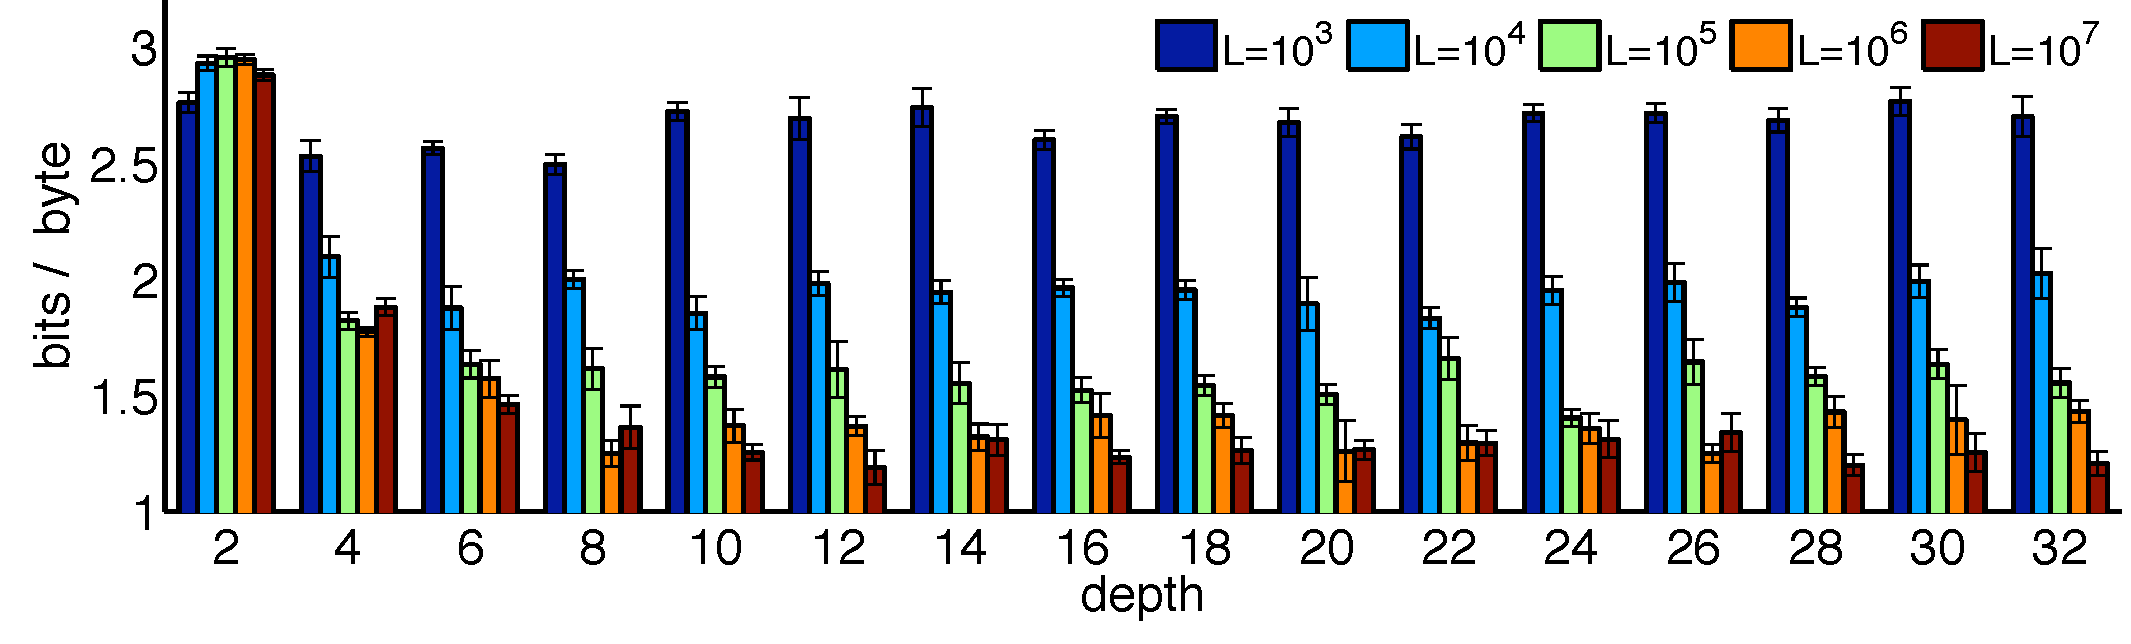
\includegraphics[width=\textwidth]{varying_depths.pdf}
%\end{center}
%\end{figure}
%A dependent HPYP can be defined though a graphical model leaf node deletion scheme.  Inference in the resulting model was shown to approximate the SM well.  \tiny{data: Calgary corpus, rests = total used nodes in 3-10 grams}
%\end{block}
\begin{figure}[htbp]
\begin{center}
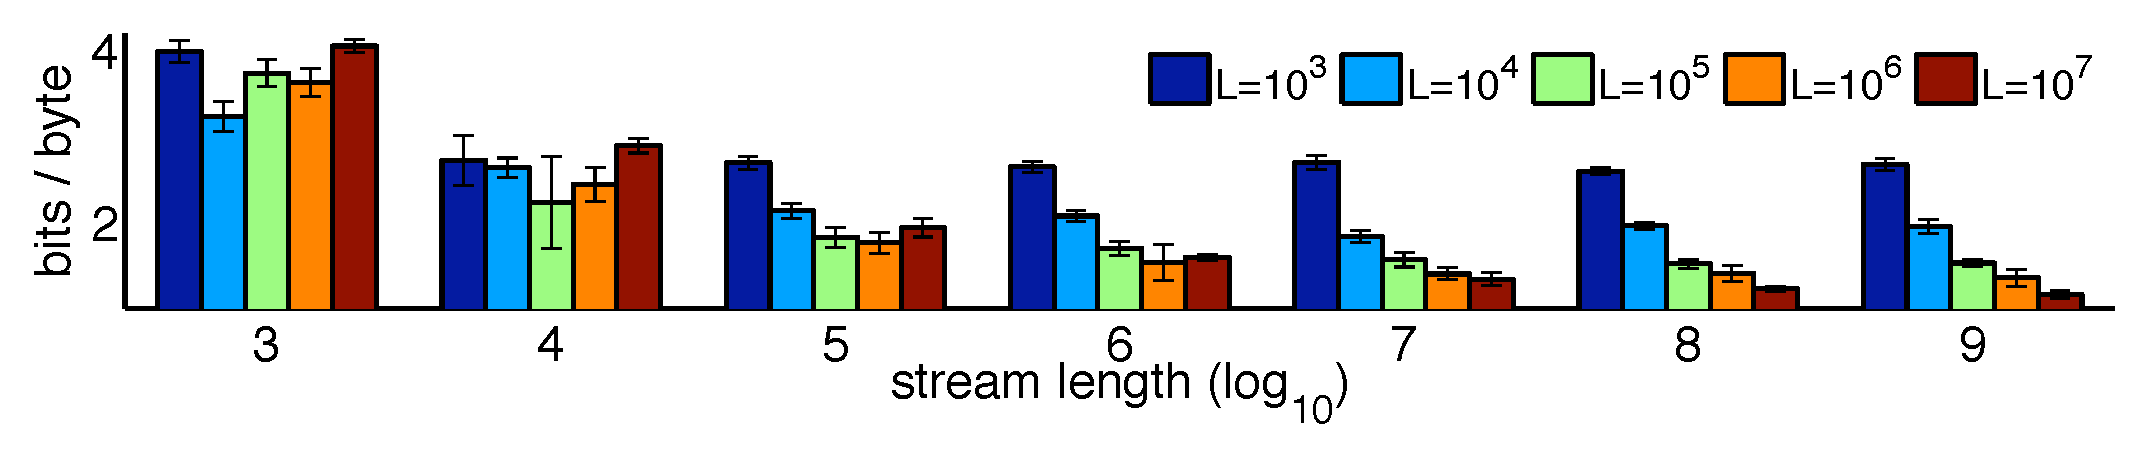
\includegraphics[width=\textwidth]{varying_stream_length.pdf}
\end{center}
\end{figure}
First streaming SM with computational asymptotics required for streaming compression.  Compressed 26.8Gb Wikipedia corpus to 4Gb (vs. 7.9Gb for gzip and 3.8Gb for PAQ).\newline
\vspace{3cm}
{\tiny $L$ is number of nodes in SM, data Wikipedia dump 2010 head, depth 16}
\end{frame}


%\subsection{Roadmap of sequence memoizer literature}
%\begin{frame}[t]{}
%Linear space sequence memoizer (SM)
%\begin{itemize}
%\item ``A Stochastic Memoizer for Sequence Data'' \cite{Wood2009}
%\item ``The Sequence Memoizer'' \cite{Wood2011}
%\end{itemize}
%SM inference
%\begin{itemize}
%\item ``A Bayesian Interpretation of Interpolated Kneser-Ney'' \citet{Teh2006}
%\item ``Hierarchical Dirichlet processes'' \cite{Teh2006b}
%\item ``A Hierarchical {B}ayesian Language Model based on {P}itman-{Y}or Processes'' \cite{Teh2006a}
%\item ``Gibbs Sampling Methods for Stick-Breaking Prior'' 



%\cite{Ishwaran2001a}
%\end{itemize}
%Constant space SM
%\begin{itemize}
%\item ``'Forgetting Counts : ... '' \cite{Bartlett2010}
%\item ``Improvements to the Sequence Memoizer'' \cite{Gasthaus2011}
%\end{itemize}
%Incremental inference
%\begin{itemize}
%\item ``Lossless compression based on the {S}equence {M}emoizer'' \cite{Gasthaus2010}
%\item ``Streaming Deplump'' \cite{Bartlett2011}
%\end{itemize}

%\end{frame}



\section{Experiments}


\subsection{Compression of byte sequences arising from arbitrary stochastic processes (computer files)}
\frame[t]
{
\begin{block}{Performance}
\begin{table}[t]
    \begin{center}
    \setlength{\tabcolsep}{1.3mm}
\begin{tabular}{l||r|c|c|c|c}
%\hline
%\multicolumn{2}{|c||}{} & \multicolumn{2}{c||}{SM} &
%\multicolumn{2}{|c|}{PPM} & CTW\\\hline
\textbf{Model} & SM & PPM & CTW & bzip2 & gzip \\\hline
%File          &  Size  &    1PF    &    UKN    &   PPM* &    PPMZ  &  CTW  \\\hline 
%\hline
%bib           & 111261 &    1.73   &{\bf 1.72}  &   1.91 &    1.74  &  1.83 \\\hline
%book1         & 768771 &{\bf 2.17}  &    2.20   &   2.40 &    2.21  &  2.18 \\\hline
%book2         & 610856 &{\bf 1.83}  &    1.84   &   2.02 &    1.87  &  1.89 \\\hline
%geo           & 102400 &{\bf 4.40}  &    4.40   &   4.83 &    4.64  &  4.53 \\\hline
%news          & 377109 &{\bf 2.20}  &    2.20   &   2.42 &    2.24  &  2.35 \\\hline
%obj1          & 21504  &{\bf 3.64}  &    3.65   &   4.00 &    3.66  &  3.72 \\\hline
%obj2          & 246814 &    2.21   &{\bf 2.19}  &   2.43 &    2.23  &  2.40 \\\hline
%paper1        & 53161  &    2.21   &{\bf 2.20}  &   2.37 &    2.22  &  2.29 \\\hline
%paper2        & 82199  &{\bf 2.18}  &    2.18   &   2.36 &    2.21  &  2.23 \\\hline
%pic           & 513216 &    0.77   &    0.82   &   0.85 &{\bf 0.76} &  0.80 \\\hline
%progc         & 39611  &    2.23   &{\bf 2.21}  &   2.40 &    2.25  &  2.33 \\\hline
%progl         & 71646  &    1.44   &{\bf 1.43}  &   1.67 &    1.46  &  1.65 \\\hline
%progp         & 49379  &    1.44   &{\bf 1.42}  &   1.62 &    1.47  &  1.68 \\\hline
%trans         & 93695  &    1.21   &{\bf 1.20}  &   1.45 &    1.23  &  1.44 \\\hline \hline
%\textbf{avg.} &        &{\bf 2.12}  &    2.12   &   2.34 &    2.16  &  2.24 \\\hline
\textbf{Average bits / byte}      &{\bf 1.89}   & 1.93  &  1.99 & 2.11 & 2.61 \\%\hline
\end{tabular}
\end{center}
\label{table:results}
\end{table}
\end{block}
Compression performance\footnote{The results for unbounded-length context PPM is from 
\cite{Cleary1997b}. The results for CTW is from \cite{Willems2009}.   The
bzip2 and gzip results come from running the corresponding standard unix
command line tools with no extra arguments.} in terms of weighted average log-loss
\[\ell(\xbf_{1:N}) = -\frac{1}{N}\sum_{i=1}^N \log_2 \EE[G(x_i|\xbf_{1:i-1})]\]
(average bits per byte under optimal entropy encoding, lower is better) for
the Calgary corpus.


}


\subsection{Language modeling}
\frame[t]
{
\begin{block}{Performance}
 \begin{table}
\begin{center}
\begin{tabular}[t]{lcc}
\hline
{\small Source } & {\small Perplexity\footnote{perplexity = $2^{\mathrm{log\; loss}}$}} \\
\hline
{\small Bengio et al.\ \cite{Bengio2003} }& 109.0 \\
%{\small Mnih \& Hinton \cite{Mnih:NIPS08} } & 112.1 \\
{\small Mnih et al.\ \cite{Mnih2009}} & \phantom{0}83.9\\
\hline
{\small 4-gram Interpolated Kneser-Ney \cite{Chen1999} }& 106.1 \\
{\small 4-gram Modified Kneser-Ney \cite{Chen1999} }& 102.4 \\
{\small 4-gram Hierarchical PYP \cite{Teh2006} } & 101.9 \\
{\small Sequence Memoizer} \cite{Wood2009}& \phantom{0}96.9\\
\hline
\end{tabular}
\end{center}
 %It has
 %been reported that the aspects of the data that are modelled by these two
 %distinct classes of models complement each other, so that even higher perfomance
 %can be achieved by combining both types of models.
 % The sequence memoizer outperforms fixed depth smoothing $n$-gram models but is bettered by a more computationally complex model on this data.  }
\label{table:ap_perplexities}
\end{table}
\end{block}
{\small Language models of an Associated Press news corpus (lower perplexity is better).  Interpolated and
 modified Kneser-Ney are state-of-the-art language models.  Provided for comparison are 
 the results for the models of Bengio et al.\ and Mnih et al.\ which belong to
 a different class of models that learn word representations from data. }
}

\subsection{Finite order Markov models vs. the sequence memoizer}
\frame[t]
{
\begin{figure}
    \includegraphics[width=.85\columnwidth]{cacm_figs/lm_results}
    \label{fig:sm_vs_ngram}
\end{figure}
 SM  versus $n^{\textrm{th}}$ order Markov models
%    $n$-gram model (solid line)
    as $n$ varies.  In red is computational
    complexity. % (for both the sequence 
%    memoizer (dashed line) and a smoothing $n$-gram model (solid line).
    %For this four million word New York Times corpus, as $n$ passes 4, the memory complexity of the Markov models grows larger than that of the sequence
   % memoizer, yet, the SM model yields modeling
   % performance that is better than all Markov models regardless of their order. %the limit of an $n$-gram as $n\rightarrow\infty$.
  %  This suggests that for $n\ge 4$ the SM model is to be preferred: it
  %  requires less space to store yet results in a comparable if not better
  %  model.
}

\section{Next}


\section{Demonstration}
\subsection{Compressor based on the sequence memoizer}
\frame[t]
{
A general purpose streaming lossless compressor (``deplump'') built on the sequence memoizer  is available for demonstration at
  \begin{itemize}
  \item \href{http://www.deplump.com/}{http://www.deplump.com/} 
  \begin{itemize}
\item    \href{http://www.deplump.com/LookupStatistics}{real time performance} 
\end{itemize}
\end{itemize}
Source code for the sequence memoizer is downloadable from 
\begin{itemize}
  \item  \href{http://www.sequencememoizer.com/}{http://www.sequencememoizer.com/} 
  \end{itemize}
}



%\section{References}

\subsection{Bibliography}
\bibliographystyle{plainnat}
	\begin{frame}[t,allowframebreaks]{}

\bibliography{../../papers/uber}
\end{frame}


%\subsection{Data: one complicated stochastic process exhibiting recency and power-law characteristics}
\begin{frame}[t]{}
\begin{figure}[t]
    \begin{center}
        \includegraphics[width=.75\columnwidth]{cacm_figs/powerlaw/freq_plot}
    \end{center}
    \label{fig:powerlaw}
\end{figure}
Power-law scaling of word frequencies in
    English text. Relative word frequency  is plotted against each words' rank when ordered according to
    frequency. There are a few very common words and a large
    number of relatively rare words. \\ {\tiny Figure from \cite{Wood2011}}.
\end{frame}	


\end{document}
